\documentclass[12pt,a4paper]{article}
\usepackage[margin=1in]{geometry}
\usepackage{amsmath,amssymb,amsfonts}
\usepackage{graphicx}
\usepackage{xcolor}
\usepackage{hyperref}
\usepackage{tcolorbox}
\usepackage{enumitem}
\usepackage{physics}
\usepackage{cleveref}
\usepackage{tikz}
\usetikzlibrary{3d,decorations.markings,arrows.meta,shapes.geometric,positioning,calc}

\hypersetup{
    colorlinks=true,
    linkcolor=blue,
    filecolor=magenta,
    urlcolor=cyan,
    citecolor=black
}

\title{Visualization of Quantum Entanglement: A Comprehensive Literature Survey}
\author{Mithilesh Kumar$^{1}$\thanks{mithilesh.kumar@krea.edu.in} and Vivek Soorya Maadoori$^{2}$\thanks{viveksoorya\_m.sias19@krea.ac.in}\\
$^{1,2}$Krea University, Sri City, Andhra Pradesh, India}
\date{\today}

\begin{document}

\maketitle

\begin{abstract}
	Quantum entanglement remains one of the most fascinating and challenging phenomena in quantum physics. As quantum systems grow in complexity, particularly in multipartite configurations, the need for effective visualization techniques becomes paramount. This literature survey provides a comprehensive review of visualization methods for quantum entanglement, spanning geometric approaches, graph-based representations, algebraic formalisms, and categorical quantum mechanics. We examine how different entanglement structures---including bipartite, multipartite, symmetric, and stabilizer states---are visualized and classified. Special attention is given to multipartite entanglement, a domain where visualization challenges are most acute due to the exponential growth of the state space. We also discuss recent advances including entanglement polytopes, hypergraph representations, ZX and ZW calculi, and tensor network visualizations. This survey synthesizes contributions from over seventy references, providing a unified perspective on the current landscape of entanglement visualization.
\end{abstract}

\bigskip

\textbf{Keywords:} Quantum Entanglement, Multipartite Entanglement, Visualization, Graph States, Stabilizer States, Majorana Representation, ZX Calculus, ZW Calculus, Entanglement Polytopes, Hypergraphs, Categorical Quantum Mechanics

\newpage

\tableofcontents

\newpage

\section{Introduction}
\label{sec:intro}

Quantum entanglement, famously termed "spooky action at a distance" by Einstein, stands as a cornerstone of quantum mechanics with profound implications for quantum information processing, quantum computation, and quantum communication. The visualization of entangled quantum states presents unique challenges, particularly as the number of parties increases. While bipartite entanglement is relatively well-understood and can be represented through simple geometric constructs such as the Bloch sphere, multipartite entanglement exhibits a rich structure that defies straightforward visualization.

The study of entanglement visualization is motivated by several practical and theoretical considerations. From a practical standpoint, visualizing entanglement structure aids in understanding complex quantum protocols, debugging quantum circuits, and developing intuition for quantum phenomena. From a theoretical perspective, visualization methods often reveal underlying mathematical structures that can lead to new insights into the nature of quantum correlations.

This survey examines the landscape of entanglement visualization methods, organizing them into several broad categories:

\begin{enumerate}
	\item \textbf{Geometric Methods}: Representations that map quantum states to geometric objects in classical spaces.
	\item \textbf{Graph-Based Methods}: Approaches using graphs, hypergraphs, and network structures to represent entanglement.
	\item \textbf{Algebraic and Categorical Methods}: Formalisms including ZX and ZW calculi that provide algebraic tools for reasoning about entanglement.
	\item \textbf{Entanglement Classification and Measures}: Methods for classifying and quantifying entanglement through polytopes, measures, and invariants.
	\item \textbf{Specialized State Classes}: Visualization approaches tailored to specific families of states such as symmetric states, stabilizer states, and Dicke states.
\end{enumerate}

Our treatment emphasizes \emph{multipartite entanglement}, where the need for visualization is most acute and where the richest variety of approaches has been developed. We draw heavily from the comprehensive survey by Anticoli et al. \cite{Undermind}, which provides an extensive overview of entanglement visualization techniques, as well as from foundational works in graph states \cite{hein2004entanglement,hein2006multiparty}, categorical quantum mechanics \cite{cqm}, and entanglement classification \cite{EntangledGraphs}.

The survey is organized as follows. We begin in \cref{sec:geometric} with geometric methods, covering the Bloch sphere, Majorana representation, coherence vectors, and phase space methods. \cref{sec:graph} examines graph-based approaches including graph states, entangled graphs, and hypergraph methods. \cref{sec:algebraic} presents algebraic and categorical methods, with detailed treatments of ZX and ZW calculi. \cref{sec:classification} discusses entanglement classification through polytopes and measures. \cref{sec:specialized} addresses specialized state classes including symmetric states, stabilizer states, and Dicke states. We conclude in \cref{sec:conclusion} with a synthesis and discussion of open problems.

Throughout this survey, we use the following notation: $N$-qubit states reside in the Hilbert space $\mathcal{H} = (\mathbb{C}^2)^{\otimes N}$. We denote pure states by $|\psi\rangle$ and mixed states by $\rho$. Bipartite splits are often denoted $(A|B)$, and multipartite partitions are written as $(A_1|A_2|\ldots|A_k)$. The reduced density matrix on subsystem $A$ is denoted $\rho_A = \text{Tr}_{\bar{A}}(\ket{\psi}\bra{\psi})$.

\section{Geometric Methods}
\label{sec:geometric}

Geometric methods for visualizing quantum entanglement map quantum states onto classical geometric objects, leveraging our intuition about familiar spaces. These approaches range from simple representations like the Bloch sphere for single qubits to more sophisticated constructions for multipartite systems.

\subsection{Bloch Sphere and Its Extensions}
\label{sec:bloch}

For single qubits, the Bloch sphere provides an elegant geometric representation where any pure state $|\psi\rangle = \cos(\theta/2)|0\rangle + e^{i\phi}\sin(\theta/2)|1\rangle$ corresponds to a point on the unit sphere in $\mathbb{R}^3$ with spherical coordinates $(\theta, \phi)$. Mixed states correspond to points inside the sphere, with the radius given by the purity $\text{Tr}(\rho^2)$.

For bipartite qubit systems, the space of states cannot be fully represented by a simple product of two Bloch spheres due to entanglement. However, the concept can be extended through various approaches. The \textbf{generalized Bloch representation} for two qubits involves a 15-dimensional parameter space, which can be projected onto lower-dimensional subspaces for visualization.

A particularly relevant extension for entanglement visualization is the \textbf{Circle Representation} \cite{circle-rep}, which uses a circle with a "radius-like" line to represent each qubit. The radius indicates the phase, while an inner color-filled circle indicates the magnitude. This representation has been extended to the \textbf{Dimensional Circle Representation} \cite{dimensional-circle}, which arranges circles representing basis states in dimensions corresponding to qubits. For three qubits, this forms a cube structure; for higher dimensions, the authors propose extending the cube structure with angled dimensions to represent additional qubits.

\subsection{Majorana Representation}
\label{sec:majorana}

The Majorana representation, originally proposed by Ettore Majorana in 1932 \cite{majorana1932atomi}, provides a powerful geometric framework for visualizing symmetric quantum states. The core idea involves representing an $N$-qubit symmetric state through $N$ points on the Bloch sphere, known as the \textbf{Majorana constellation}.

Given a symmetric state $|\psi\rangle$ in $(\mathbb{C}^2)^{\otimes N}$, we can project it onto spin-coherent states. The state can be written as:
\begin{equation}
	|\psi\rangle = \mathcal{N} \sum_{k=0}^{N} c_k |N/2, k - N/2\rangle,
\end{equation}
where $|N/2, m\rangle$ are Dicke states (see \cref{sec:dicke}), and the coefficients $c_k$ determine the Majorana constellation. Each point in the constellation corresponds to a zero of the polynomial $P(z) = \sum_{k=0}^{N} (-1)^{N-k} c_k z^k$, representing the roots of the Majorana polynomial.

The Majorana representation has proven particularly valuable for:
\begin{itemize}
	\item Visualizing the entanglement structure of symmetric states
	\item Classifying symmetric entangled states
	\item Understanding the geometric phase of multipartite states
	\item Studying the stability of entanglement under perturbations
\end{itemize}

For example, the $W$ state $|W_N\rangle = \frac{1}{\sqrt{N}}(|10\ldots 0\rangle + |01\ldots 0\rangle + \cdots + |00\ldots 1\rangle)$ has a Majorana constellation consisting of $N-1$ points at the north pole and one point at the south pole. The GHZ state $|\text{GHZ}_N\rangle = \frac{1}{\sqrt{2}}(|0\rangle^{\otimes N} + |1\rangle^{\otimes N})$ has two points at opposite poles.

The Majorana representation connects naturally to the \textbf{stereographic projection}, where points on the Bloch sphere are mapped to the complex plane. This mapping provides an intuitive visualization of how changes in the quantum state correspond to movements of points on the sphere.

A variant called the \textbf{Bloch-Norm Representation} combines Bloch vectors with the Majorana constellation to provide a geometric characterization of different entanglement classes in three-qubit systems. This approach naturally leads to bounds between the tangle and the norm of a vector, providing geometric insight into the structure of tripartite entanglement.

\subsection{Coherence Vector Representation}
\label{sec:coherence}

The coherence vector (or generalized Bloch vector) provides an alternative geometric representation that generalizes the Bloch sphere to higher dimensions. For an $N$-qubit system, the coherence vector resides in $\mathbb{R}^{4^N - 1}$ and encodes all correlation functions.

For a single qubit, the Bloch vector $\vec{r} = (\langle X \rangle, \langle Y \rangle, \langle Z \rangle)$ completely characterizes the state. For multipartite systems, we consider the full collection of $k$-party correlation functions for all $k = 1, \ldots, N$. The coherence vector representation has been used to visualize entanglement through the study of correlation polytopes \cite{EntangledGraphs}.

One advantage of the coherence vector approach is its direct connection to measurable quantities---expectation values of Pauli operators. This makes it particularly suitable for experimental contexts where tomography is performed through Pauli measurements.

However, the exponential growth of the representation space ($4^N - 1$ dimensions for $N$ qubits) limits practical visualization to small $N$. For $N = 2$, the 15-dimensional space can be projected onto lower-dimensional subspaces to reveal interesting features; for $N \geq 3$, numerical methods and dimensionality reduction become essential.

\subsection{Phase Space Methods}
\label{sec:phase-space}

Phase space methods provide alternative geometric representations by mapping quantum states to functions on classical phase spaces. These approaches are particularly natural for continuous-variable systems but have also been adapted to discrete systems.

For qubits, one can consider phase space representations based on:
\begin{itemize}
	\item \textbf{Torus knots}: The quasicrystal approach represents qubit states as points on a torus, with entanglement manifested as linking patterns in the visualization \cite{Undermind}.
	\item \textbf{Quasi-probability distributions}: The discrete Wigner function provides a phase space representation for qudit systems. Negative quasi-probabilities are indicative of non-classicality and entanglement.
	\item \textbf{Poincaré spheres}: For optical systems, the Poincaré sphere provides a natural representation of polarization states, which can be extended to represent entanglement through composite spheres.
\end{itemize}

The Great Deluge Algorithm provides an interesting approach to visualizing the "entanglement landscape" by mapping states to a high-dimensional space and projecting down to visualize the distribution of entanglement across the state space. This method has been applied to understand the structure of multipartite entanglement and identify highly entangled states.

Hypertrees offer another geometric approach, representing the entanglement structure as a hierarchical tree where nodes correspond to bipartitions and edge weights represent entanglement measures. This approach is particularly natural for understanding hierarchical entanglement structure in tensor network states.

\begin{figure}[htbp]
	\centering
	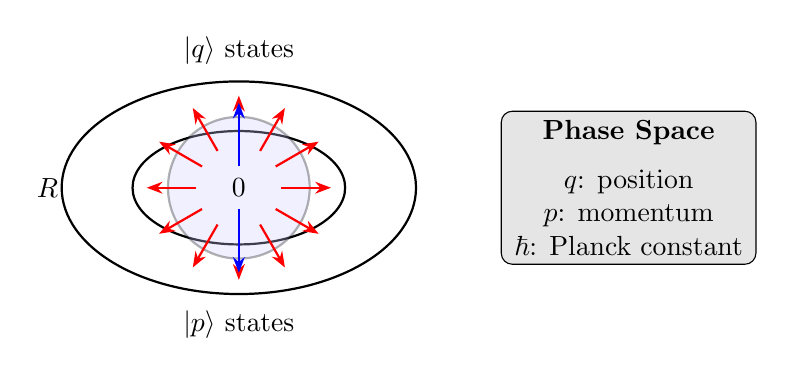
\begin{tikzpicture}[scale=0.9]
		\draw[thick] (0,0) ellipse (2.5cm and 1.5cm);
		\draw[thick] (0,0) ellipse (1.5cm and 0.8cm);
		\draw[thick, fill=blue!20, opacity=0.3] (0,0) circle (1cm);

		\foreach \angle in {0,30,...,330} {
		\draw[thick, red, -{Stealth[length=2mm]}] ({\angle}:0.6cm) -- ({\angle}:1.3cm);
		}

		\draw[thick, blue, -{Stealth[length=2mm]}] (0,0.3) -- (0,1.2);
		\draw[thick, blue, -{Stealth[length=2mm]}] (0,-0.3) -- (0,-1.2);

		\node[above] at (0,1.6) {$|q\rangle$ states};
		\node[below] at (0,-1.6) {$|p\rangle$ states};
		\node at (-2.7,0) {$R$};
		\node at (0,0) {$0$};

		\node[draw, rounded corners, fill=gray!20] at (5.5,0) {
			\begin{minipage}{3cm}
				\centering
				\textbf{Phase Space}\\ \vspace{0.2cm}
				$q$: position\\
				$p$: momentum\\
				$\hbar$: Planck constant
			\end{minipage}
		};
	\end{tikzpicture}
	\caption{Phase space representation for continuous-variable quantum systems. The torus structure arises from periodic boundary conditions in position ($q$) and momentum ($p$) spaces.}
	\label{fig:phase-space-torus}
\end{figure}

\begin{figure}[htbp]
	\centering
	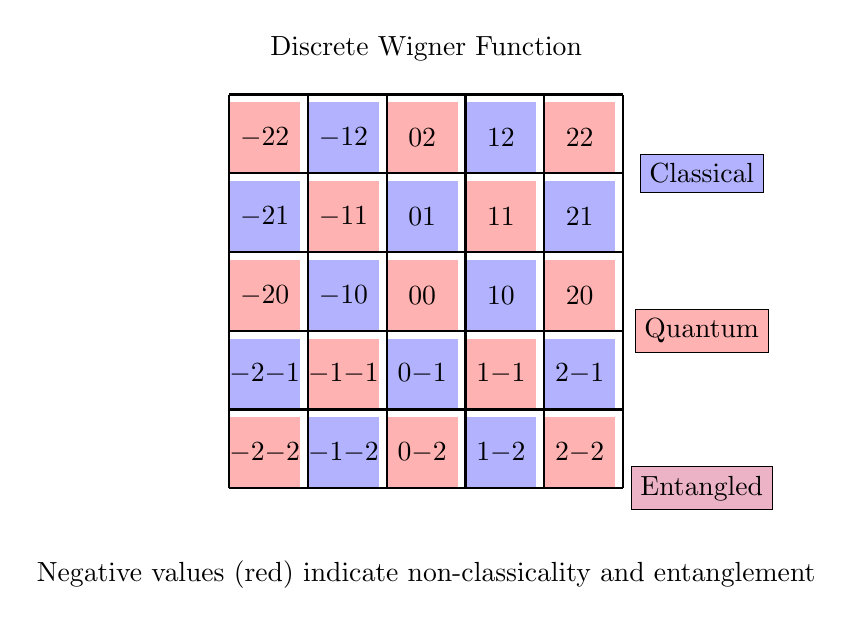
\begin{tikzpicture}
		\foreach \x in {-2,-1,0,1,2} {
				\foreach \y in {-2,-1,0,1,2} {
						\pgfmathparse{\x+\y}
						\ifodd \pgfmathresult
							\fill[blue!30] (\x*1cm,\y*1cm) rectangle ++(0.9cm,0.9cm);
						\else
							\fill[red!30] (\x*1cm,\y*1cm) rectangle ++(0.9cm,0.9cm);
						\fi
						\node at (\x*1cm+0.45cm,\y*1cm+0.45cm) {\pgfmathprintnumber{\x}\pgfmathprintnumber{\y}};
					}
			}
		\draw[thick] (-2cm,-2cm) grid (3cm,3cm);

		\node[draw, fill=blue!30, minimum width=1.5cm] at (4,2) {Classical};
		\node[draw, fill=red!30, minimum width=1.5cm] at (4,0) {Quantum};
		\node[draw, fill=purple!30, minimum width=1.5cm] at (4,-2) {Entangled};

		\node[above] at (0.5,3.3) {Discrete Wigner Function};
		\node[below] at (0.5,-2.8) {Negative values (red) indicate non-classicality and entanglement};
	\end{tikzpicture}
	\caption{Discrete Wigner function for a qubit system. Each cell represents a phase space cell, with colors indicating quasi-probability values. Negative values (red) signal non-classicality.}
	\label{fig:wigner-function}
\end{figure}

\begin{figure}[htbp]
	\centering
	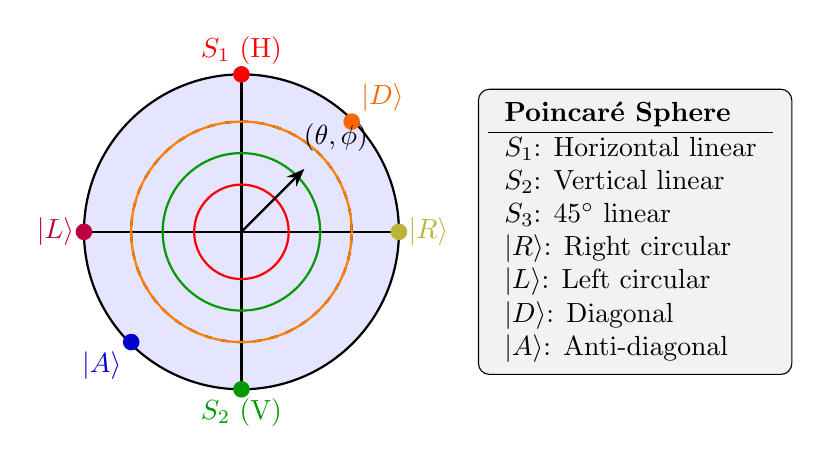
\begin{tikzpicture}
		\draw[thick, fill=blue!10] (0,0) circle (2cm);
		\draw[thick, dashed] (0,0) circle (1.4cm);
		\draw[thick] (0,-2) -- (0,2);
		\draw[thick] (-2,0) -- (2,0);

		\foreach \r/\col in {0.6/red, 1.0/green!60!black, 1.4/orange} {
				\draw[\col, thick] (0,0) circle (\r);
			}

		\fill[red] (0,2) circle (3pt) node[above] {$S_1$ (H)};
		\fill[green!60!black] (0,-2) circle (3pt) node[below] {$S_2$ (V)};
		\fill[yellow!70!black] (2,0) circle (3pt) node[right] {$|R\rangle$};
		\fill[purple] (-2,0) circle (3pt) node[left] {$|L\rangle$};
		\fill[orange!80!red] (1.4,1.4) circle (3pt) node[above right] {$|D\rangle$};
		\fill[blue!80!black] (-1.4,-1.4) circle (3pt) node[below left] {$|A\rangle$};

		\draw[-Stealth, thick] (0,0) -- (0.8,0.8);
		\node at (1.2,1.2) {$(\theta,\phi)$};

		\node[draw, rounded corners, fill=gray!10, align=left] at (5,0) {
			\begin{tabular}{l}
				\textbf{Poincaré Sphere}    \\
				\hline
				$S_1$: Horizontal linear    \\
				$S_2$: Vertical linear      \\
				$S_3$: $45^\circ$ linear    \\
				$|R\rangle$: Right circular \\
				$|L\rangle$: Left circular  \\
				$|D\rangle$: Diagonal       \\
				$|A\rangle$: Anti-diagonal
			\end{tabular}
		};
	\end{tikzpicture}
	\caption{Poincaré sphere representing polarization states of light. Each point on the sphere surface corresponds to a unique polarization state. For bipartite entanglement, composite Poincaré spheres can represent two-photon states.}
	\label{fig:poincare-sphere}
\end{figure}

\begin{figure}[htbp]
	\centering
	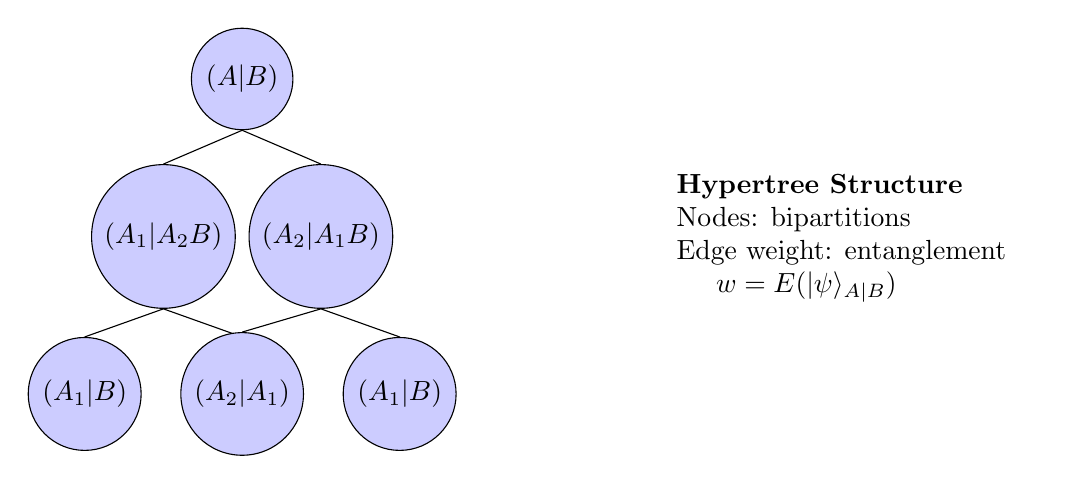
\begin{tikzpicture}[
			level distance=2cm,
			sibling distance=2cm,
			edge from parent path={(\tikzparentnode.south) -- (\tikzchildnode.north)},
			every node/.style={draw, circle, fill=blue!20, minimum size=1cm}
		]
		\node {$(A|B)$}
		child {
				node {$(A_1|A_2B)$}
				child {
						node {$(A_1|B)$}
					}
				child {
						node {$(A_2|B)$}
					}
			}
		child {
				node {$(A_2|A_1B)$}
				child {
						node {$(A_2|A_1)$}
					}
				child {
						node {$(A_1|B)$}
					}
			};

		\node[draw=none, fill=none, right=1cm] at (4,-2) {
			\begin{tabular}{l}
				\textbf{Hypertree Structure} \\
				Nodes: bipartitions          \\
				Edge weight: entanglement    \\
				\hspace{0.5cm}$w = E(|\psi\rangle_{A|B})$
			\end{tabular}
		};
	\end{tikzpicture}
	\caption{Hypertree representation of multipartite entanglement. Each node represents a bipartition of the system, and edge weights quantify the entanglement across that cut. This hierarchical structure reveals the nesting of entanglement in tensor network states.}
	\label{fig:hypertree}
\end{figure}

\begin{figure}[htbp]
	\centering
	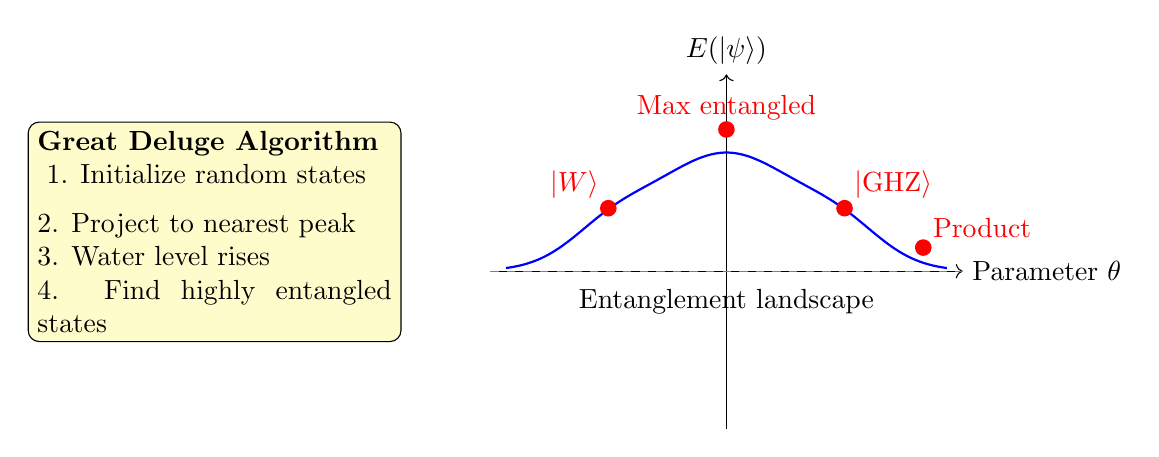
\begin{tikzpicture}
		\draw[->] (-3,0) -- (3,0) node[right] {Parameter $\theta$};
		\draw[->] (0,-2) -- (0,2.5) node[above] {$E(|\psi\rangle)$};

		\draw[thick, blue, domain=-2.8:2.8, samples=100] plot (\x, {1.5*exp(-\x*\x/2) + 0.3*exp(-(\x-1.5)*(\x-1.5)/0.5) + 0.3*exp(-(\x+1.5)*(\x+1.5)/0.5)});

		\fill[red] (1.5,0.8) circle (3pt) node[above right] {$|\text{GHZ}\rangle$};
		\fill[red] (-1.5,0.8) circle (3pt) node[above left] {$|W\rangle$};
		\fill[red] (0,1.8) circle (3pt) node[above] {Max entangled};
		\fill[red] (2.5,0.3) circle (3pt) node[above right] {Product};

		\draw[dashed, gray] (-3,0) -- (3,0);
		\node[below] at (0,-0.1) {Entanglement landscape};

		\node[draw, rounded corners, fill=yellow!20] at (-6.5,0.5) {
			\begin{minipage}{4.5cm}
				\textbf{Great Deluge Algorithm}\\
				\vspace{0.2cm}
				1. Initialize random states\\
				2. Project to nearest peak\\
				3. Water level rises\\
				4. Find highly entangled states
			\end{minipage}
		};
	\end{tikzpicture}
	\caption{Entanglement landscape visualization using the Great Deluge Algorithm. Peaks correspond to highly entangled states (GHZ, W), valleys to product states. The algorithm floods this landscape to identify maximally entangled configurations.}
	\label{fig:entanglement-landscape}
\end{figure}

\section{Graph-Based Methods}
\label{sec:graph}

Graph-based methods represent quantum states through network structures, where vertices correspond to quantum systems (qubits, qudits) and edges represent correlations or entanglement. These methods have proven remarkably fruitful, particularly for stabilizer states and certain classes of multipartite entanglement.

\subsection{Graph States}
\label{sec:graph-states}

Graph states represent a fundamental class of multipartite entangled states that can be described compactly by graphs. Given an undirected graph $G = (V, E)$ with vertex set $V$ and edge set $E$, the corresponding graph state $|G\rangle$ is defined by:
\begin{equation}
	|G\rangle = \prod_{(a,b) \in E} U_{ab} |+\rangle^{\otimes |V|},
\end{equation}
where $U_{ab} = \text{diag}(1, 1, 1, -1)$ is the controlled-$Z$ gate acting on qubits $a$ and $b$, and $|+\rangle = \frac{1}{\sqrt{2}}(|0\rangle + |1\rangle)$ is the Hadamard eigenstate.

\begin{figure}[htbp]
	\centering
	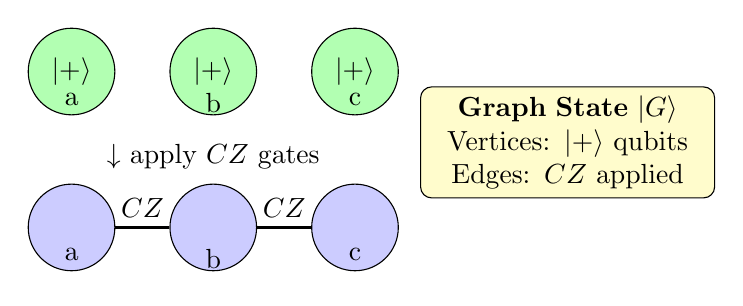
\begin{tikzpicture}[scale=0.9]
		\node[draw, circle, fill=green!30, minimum size=1.1cm] (a) at (0,0) {$|+\rangle$};
		\node[draw, circle, fill=green!30, minimum size=1.1cm] (b) at (2,0) {$|+\rangle$};
		\node[draw, circle, fill=green!30, minimum size=1.1cm] (c) at (4,0) {$|+\rangle$};

		\node[below=0.15cm] at (a) {a};
		\node[below=0.15cm] at (b) {b};
		\node[below=0.15cm] at (c) {c};

		\node[thick] at (2,-1.2) {$\downarrow$ apply $CZ$ gates};

		\node[draw, circle, fill=blue!20, minimum size=1.1cm] (a2) at (0,-2.2) {};
		\node[draw, circle, fill=blue!20, minimum size=1.1cm] (b2) at (2,-2.2) {};
		\node[draw, circle, fill=blue!20, minimum size=1.1cm] (c2) at (4,-2.2) {};

		\node[below=0.15cm] at (a2) {a};
		\node[below=0.15cm] at (b2) {b};
		\node[below=0.15cm] at (c2) {c};

		\draw[thick] (a2) -- node[above] {$CZ$} (b2);
		\draw[thick] (b2) -- node[above] {$CZ$} (c2);

		\node[draw, rounded corners, fill=yellow!20, text width=3.5cm, align=center] at (7,-1) {
			\textbf{Graph State $|G\rangle$}\\
			Vertices: $|+\rangle$ qubits\\
			Edges: $CZ$ applied
		};
	\end{tikzpicture}
	\caption{Construction of a graph state from a graph $G$. Each vertex represents a qubit initialized in $|+\rangle$, and each edge represents a controlled-$Z$ entangling operation applied between connected qubits.}
	\label{fig:graph-state-construction}
\end{figure}



Each graph state has a beautiful interpretation: vertices represent qubits prepared in the $|+\rangle$ state, and edges represent the application of entangling $CZ$ gates. The resulting state exhibits genuine multipartite entanglement and serves as a universal resource for measurement-based quantum computation.

The relationship between graph structure and entanglement properties is rich:
\begin{itemize}
	\item \textbf{Connectivity and entanglement}: More connected graphs generally support more robust multipartite entanglement.
	\item \textbf{Cluster states}: The 2D square lattice graph gives the famous cluster state, which is a universal resource for one-way quantum computation.
	\item \textbf{Star graphs}: Produce highly symmetric states with applications in quantum networking.
	\item \textbf{Graph connectivity and entanglement depth}: The maximum genuine entanglement depth achievable in a graph state is related to the graph's connectivity.
\end{itemize}

\begin{figure}[htbp]
	\centering
	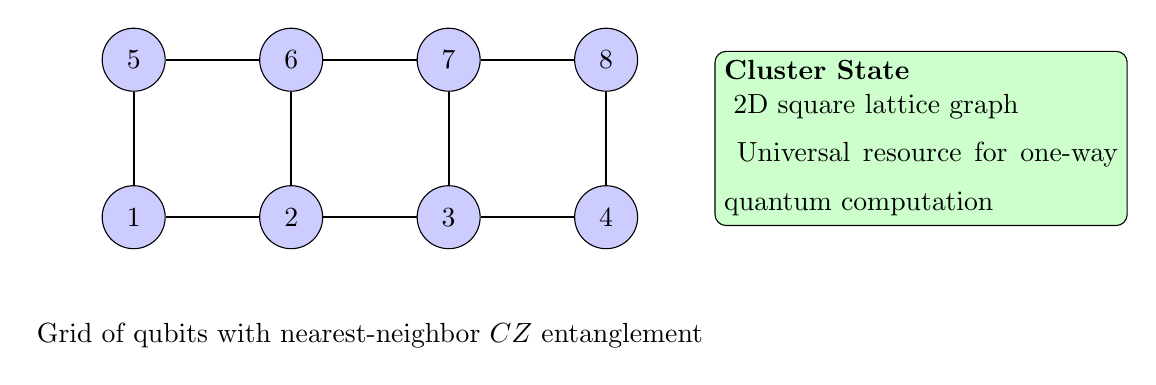
\begin{tikzpicture}
		\node[draw, circle, fill=blue!20, minimum size=0.8cm] (11) at (0,0) {1};
		\node[draw, circle, fill=blue!20, minimum size=0.8cm] (12) at (2,0) {2};
		\node[draw, circle, fill=blue!20, minimum size=0.8cm] (13) at (4,0) {3};
		\node[draw, circle, fill=blue!20, minimum size=0.8cm] (14) at (6,0) {4};
		\node[draw, circle, fill=blue!20, minimum size=0.8cm] (21) at (0,2) {5};
		\node[draw, circle, fill=blue!20, minimum size=0.8cm] (22) at (2,2) {6};
		\node[draw, circle, fill=blue!20, minimum size=0.8cm] (23) at (4,2) {7};
		\node[draw, circle, fill=blue!20, minimum size=0.8cm] (24) at (6,2) {8};

		\draw[thick] (11) -- (12) -- (13) -- (14);
		\draw[thick] (21) -- (22) -- (23) -- (24);
		\draw[thick] (11) -- (21);
		\draw[thick] (12) -- (22);
		\draw[thick] (13) -- (23);
		\draw[thick] (14) -- (24);

		\node[draw, rounded corners, fill=green!20] at (10,1) {
			\begin{minipage}{5cm}
				\textbf{Cluster State}\\
				\vspace{0.2cm}
				2D square lattice graph\\
				\vspace{0.2cm}
				Universal resource for one-way quantum computation
			\end{minipage}
		};

		\node at (3,-1.5) {Grid of qubits with nearest-neighbor $CZ$ entanglement};
	\end{tikzpicture}
	\caption{The cluster state, a 2D square lattice graph state. This is a universal resource for measurement-based quantum computation, where computation proceeds through single-qubit measurements on the entangled cluster.}
	\label{fig:cluster-state}
\end{figure}

\begin{figure}[htbp]
	\centering
	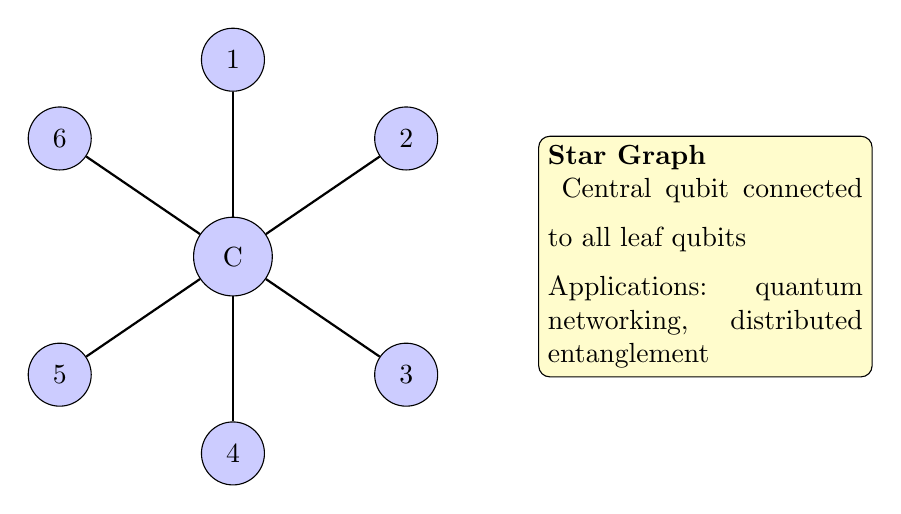
\begin{tikzpicture}
		\node[draw, circle, fill=blue!20, minimum size=1cm] (center) at (0,0) {C};
		\node[draw, circle, fill=blue!20, minimum size=0.8cm] (1) at (0,2.5) {1};
		\node[draw, circle, fill=blue!20, minimum size=0.8cm] (2) at (2.2,1.5) {2};
		\node[draw, circle, fill=blue!20, minimum size=0.8cm] (3) at (2.2,-1.5) {3};
		\node[draw, circle, fill=blue!20, minimum size=0.8cm] (4) at (0,-2.5) {4};
		\node[draw, circle, fill=blue!20, minimum size=0.8cm] (5) at (-2.2,-1.5) {5};
		\node[draw, circle, fill=blue!20, minimum size=0.8cm] (6) at (-2.2,1.5) {6};

		\draw[thick] (center) -- (1);
		\draw[thick] (center) -- (2);
		\draw[thick] (center) -- (3);
		\draw[thick] (center) -- (4);
		\draw[thick] (center) -- (5);
		\draw[thick] (center) -- (6);

		\node[draw, rounded corners, fill=yellow!20] at (6,0) {
			\begin{minipage}{4cm}
				\textbf{Star Graph}\\
				\vspace{0.2cm}
				Central qubit connected to all leaf qubits\\[0.2cm]
				Applications: quantum networking, distributed entanglement
			\end{minipage}
		};
	\end{tikzpicture}
	\caption{Star graph configuration. The central qubit (C) is connected to all leaf qubits. Star graph states are highly symmetric and useful for quantum networking protocols where entanglement needs to be distributed from a central node.}
	\label{fig:star-graph}
\end{figure}



The \textbf{GraphStateVis} tool \cite{GraphStateVis} provides an interactive web-based platform for visualizing graph states and their stabilizer groups. This tool enables:
\begin{itemize}
	\item Interactive construction of graphs
	\item Visualization of Pauli-weight distributions in stabilizer operators
	\item Analysis of entanglement criteria and noise thresholds
	\item Exploration of graph-state properties in the context of near-term quantum algorithms
\end{itemize}

Local complementation (LC) provides a key operation: applying LC on a vertex $v$ inverts the connectivity between all neighbors of $v$. Graph states that are equivalent under LC (or LC plus edge deletion/addition, denoted LCE) have the same entanglement properties. This classification has been extensively studied, with complete classification available up to 12 qubits \cite{hein2004entanglement,danielsen2008graph}.

\begin{figure}[htbp]
	\centering
	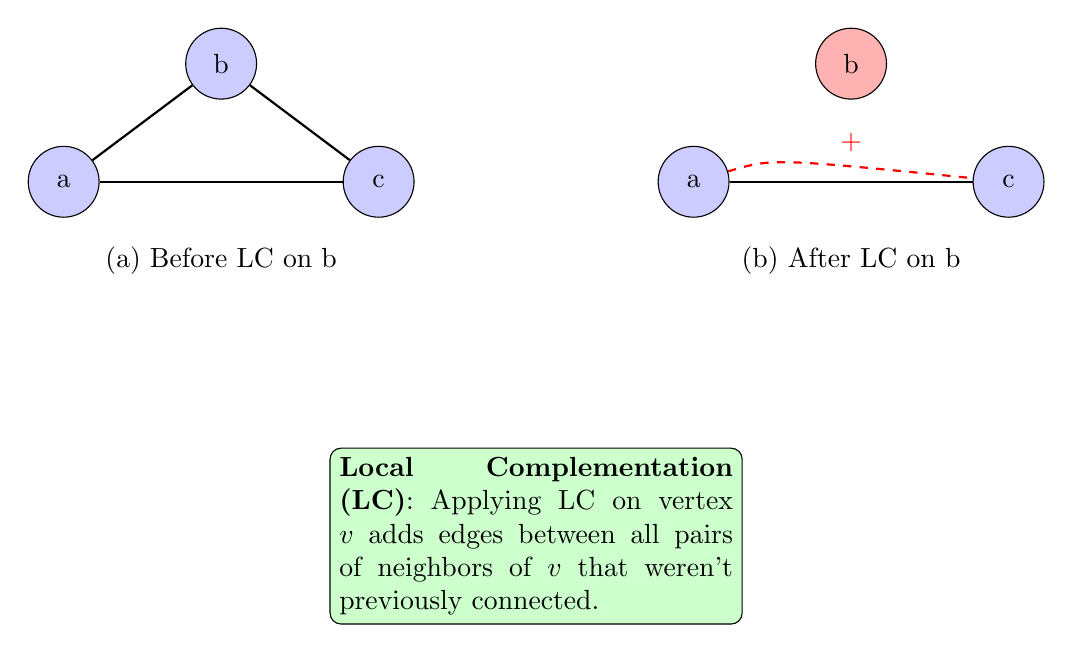
\begin{tikzpicture}
		\node[draw, circle, fill=blue!20, minimum size=0.9cm] (a) at (0,0) {a};
		\node[draw, circle, fill=blue!20, minimum size=0.9cm] (b) at (2,1.5) {b};
		\node[draw, circle, fill=blue!20, minimum size=0.9cm] (c) at (4,0) {c};

		\draw[thick] (a) -- (b);
		\draw[thick] (b) -- (c);
		\draw[thick] (a) -- (c);

		\node at (2,-1) {(a) Before LC on b};

		\node[draw, circle, fill=blue!20, minimum size=0.9cm] (a2) at (8,0) {a};
		\node[draw, circle, fill=red!30, minimum size=0.9cm] (b2) at (10,1.5) {b};
		\node[draw, circle, fill=blue!20, minimum size=0.9cm] (c2) at (12,0) {c};

		\draw[thick] (a2) -- (c2);
		\draw[dashed, red, thick] (a2) .. controls (9,0.3) .. (c2);
		\draw[red] (10,0.5) node {$+$};

		\node at (10,-1) {(b) After LC on b};

		\node[draw, rounded corners, fill=green!20] at (6,-4.5) {
			\begin{minipage}{5cm}
				\textbf{Local Complementation (LC)}: Applying LC on vertex $v$ adds edges between all pairs of neighbors of $v$ that weren't previously connected.
			\end{minipage}
		};
	\end{tikzpicture}
	\caption{Illustration of local complementation on a graph state. When LC is applied to vertex $b$, an edge is added between its neighbors $a$ and $c$. States related by LC (and edge additions/deletions) have equivalent entanglement structure.}
	\label{fig:local-complementation}
\end{figure}

The \textbf{stabilizer formalism} provides a powerful algebraic description of graph states. The stabilizer group $\mathcal{S}$ is generated by $N$ independent operators, each of which has $|G\rangle$ as a +1 eigenvector. The stabilizer generators can be read directly from the graph structure.

Elliott, Eastin, and Caves developed a \textbf{graphical description of stabilizer states} that provides intuitive understanding of how Clifford operations and Pauli measurements affect graph states. This work complements the algebraic approach with visual intuition.

Recent work explores entanglement in pseudo-graph states using the Entanglement Distance (ED) measure, demonstrating how vertex degree distribution determines entanglement properties. This highlights the topological character of entanglement in graph states.

Recent work extends the framework to directed graphs, relating multipartite entanglement to local connectivity through measures derived from the Fubini-Study metric. This demonstrates that vertex degree distribution fully determines certain entanglement measures, revealing topological invariance.

Stabilizer states and graph states have been further connected to:
\begin{itemize}
	\item \textbf{Quantum error correction}: Graph codes provide a natural framework for stabilizer codes.
	\item \textbf{Quantum networks}: Graph states serve as entanglement resources in quantum routing protocols.
	\item \textbf{Classical codes}: Recent work shows connections between classical error-correcting codes and k-UNI (k-uniform) and AME (Absolutely Maximally Entangled) states \cite{Raissi2021}.
\end{itemize}





\begin{figure}[htbp]
	\centering
	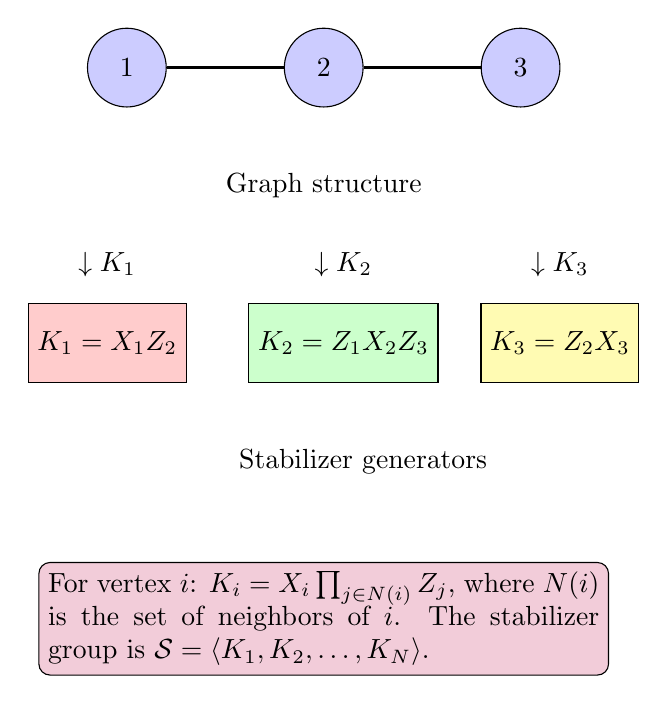
\begin{tikzpicture}
		\node[draw, circle, fill=blue!20, minimum size=1cm] (1) at (-1,0) {1};
		\node[draw, circle, fill=blue!20, minimum size=1cm] (2) at (1.5,0) {2};
		\node[draw, circle, fill=blue!20, minimum size=1cm] (3) at (4,0) {3};

		\draw[thick] (1) -- (2) -- (3);

		\node at (1.5,-1.5) {Graph structure};

		\node at (-1.25,-2.5) {$\downarrow K_1$};
		\node at (1.75,-2.5) {$\downarrow K_2$};
		\node at (4.5,-2.5) {$\downarrow K_3$};

		\node[draw, rectangle, fill=red!20, minimum height=1cm] at (-1.25,-3.5) {$K_1 = X_1 Z_2$};
		\node[draw, rectangle, fill=green!20, minimum height=1cm] at (1.75,-3.5) {$K_2 = Z_1 X_2 Z_3$};
		\node[draw, rectangle, fill=yellow!30, minimum height=1cm] at (4.5,-3.5) {$K_3 = Z_2 X_3$};

		\node at (2.0,-5) {Stabilizer generators};

		\node[draw, rounded corners, fill=purple!20] at (1.5,-7) {
			\begin{minipage}{7cm}
				For vertex $i$: $K_i = X_i \prod_{j \in N(i)} Z_j$, where $N(i)$ is the set of neighbors of $i$. The stabilizer group is $\mathcal{S} = \langle K_1, K_2, \ldots, K_N \rangle$.
			\end{minipage}
		};
	\end{tikzpicture}
	\caption{Reading stabilizer generators from the graph structure. For each vertex $i$, the stabilizer generator $K_i$ is the product of $X$ on vertex $i$ and $Z$ on all its neighbors. These $N$ operators generate the full stabilizer group of $2^N$ elements.}
	\label{fig:stabilizer-generators}
\end{figure}

\begin{figure}[htbp]
	\centering
	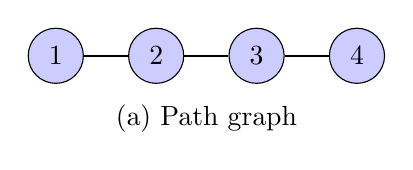
\begin{tikzpicture}[scale=0.85]
		\node[draw, circle, fill=blue!20, minimum size=0.7cm] (1) at (0,0) {1};
		\node[draw, circle, fill=blue!20, minimum size=0.7cm] (2) at (1.5,0) {2};
		\node[draw, circle, fill=blue!20, minimum size=0.7cm] (3) at (3,0) {3};
		\node[draw, circle, fill=blue!20, minimum size=0.7cm] (4) at (4.5,0) {4};
		\draw[thick] (1) -- (2) -- (3) -- (4);
		\node[below=0.5cm] at (2.25,0) {(a) Path graph};
	\end{tikzpicture}

	\vspace{0.5cm}

	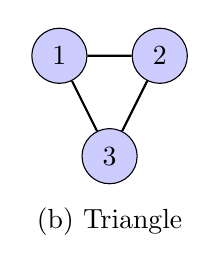
\begin{tikzpicture}[scale=0.85]
		\node[draw, circle, fill=blue!20, minimum size=0.7cm] (c1) at (0,1) {1};
		\node[draw, circle, fill=blue!20, minimum size=0.7cm] (c2) at (1.5,1) {2};
		\node[draw, circle, fill=blue!20, minimum size=0.7cm] (c3) at (0.75,-0.5) {3};
		\draw[thick] (c1) -- (c2) -- (c3) -- (c1);
		\node[below=1.8cm] at (0.75,1) {(b) Triangle};
	\end{tikzpicture}

	\vspace{0.5cm}

	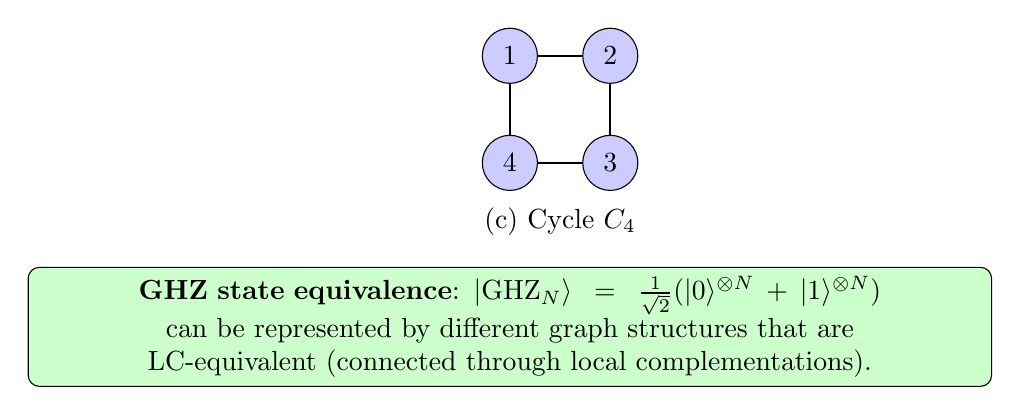
\begin{tikzpicture}[scale=0.85]
		\node[draw, circle, fill=blue!20, minimum size=0.7cm] (s1) at (0,0.8) {1};
		\node[draw, circle, fill=blue!20, minimum size=0.7cm] (s2) at (1.5,0.8) {2};
		\node[draw, circle, fill=blue!20, minimum size=0.7cm] (s3) at (1.5,-0.8) {3};
		\node[draw, circle, fill=blue!20, minimum size=0.7cm] (s4) at (0,-0.8) {4};
		\draw[thick] (s1) -- (s2) -- (s3) -- (s4) -- (s1);
		\node[below=1.8cm] at (0.75,0.8) {(c) Cycle $C_4$};


		\node[draw, rounded corners, fill=green!20, text width=12cm, align=center, below=2cm] {
			\textbf{GHZ state equivalence}: $|\text{GHZ}_N\rangle = \frac{1}{\sqrt{2}}(|0\rangle^{\otimes N} + |1\rangle^{\otimes N})$ can be represented by different graph structures that are LC-equivalent (connected through local complementations).
		};
	\end{tikzpicture}

	\vspace{0.3cm}
	\caption{Different graph representations of the GHZ state. The GHZ state can be represented as a path graph, cycle graph, or other connected structures, all of which are locally complemented to each other and thus share equivalent entanglement properties.}
	\label{fig:ghz-graph-equivalence}
\end{figure}

\subsection{Entangled Graphs}
\label{sec:entangled-graphs}

While graph states use graphs as a constructive tool, the \textbf{entangled graphs} approach of Gharahi and Akhtarshenas \cite{EntangledGraphs} uses graphs as a \emph{classification} tool for arbitrary multipartite states. This approach represents the entanglement structure of multi-qubit systems through weighted graphs.

The key ideas are:
\begin{enumerate}
	\item \textbf{Nodes represent qubits}: Each vertex in the graph corresponds to one qubit in the system.
	\item \textbf{Weighted edges represent bipartite entanglement}: The weight of an edge between qubits $i$ and $j$ is given by the \textbf{concurrence} $C_{ij}$, a measure of bipartite entanglement:
	      \begin{equation}
		      C_{ij} = \max(0, \lambda_1 - \lambda_2 - \lambda_3 - \lambda_4),
	      \end{equation}
	      where $\lambda_i$ are the square roots of the eigenvalues of $\rho_{ij}\tilde{\rho}_{ij}$, with $\tilde{\rho}_{ij} = (\sigma_y \otimes \sigma_y) \rho_{ij}^* (\sigma_y \otimes \sigma_y)$.
	\item \textbf{Enclosing circles represent global entanglement}: A circle enclosing a subset of nodes indicates that those qubits share genuine multipartite entanglement that cannot be reduced to bipartite entanglement alone.
\end{enumerate}

This representation has proven particularly valuable for classifying 4-qubit entanglement, where the authors identified the complete classification of states under stochastic local operations and classical communication (SLOCC). The entangled graph method reveals the hierarchy of entanglement in 4-qubit states, distinguishing between different types of genuine 4-partite entanglement.

For example, consider the 4-qubit state:
\begin{equation}
	|\psi\rangle = \frac{1}{\sqrt{2}}(|0000\rangle + |1111\rangle),
\end{equation}
which has maximum concurrence between all pairs. This would be represented as a complete graph $K_4$ with all edges weighted 1, and all four vertices enclosed in a circle to indicate global entanglement.

In contrast, the state:
\begin{equation}
	|\psi\rangle = \frac{1}{\sqrt{2}}(|0000\rangle + |1100\rangle),
\end{equation}
has only bipartite entanglement between qubits 1-2 and 3-4, with no global entanglement. This would be represented as two disconnected edges with weight 1, no enclosing circles.

The method can be extended to larger systems, though the combinatorial complexity grows rapidly. The approach provides an intuitive visual language for communicating entanglement structure.

A related approach using \textbf{spanning graphs} was developed for studying entanglement spreading in hybrid quantum circuits with measurements \cite{SpanningGraphs2025}. This graphical representation allows identification of the evolution of genuine multipartite entanglement in general subregions, with minimal spanning graphs connecting various parties.

\subsection{Hypergraph Methods}
\label{sec:hypergraphs}

Hypergraphs extend ordinary graphs by allowing edges (called hyperedges) to connect more than two vertices. This makes them natural candidates for representing multipartite entanglement, where correlations can involve more than two parties.

Anticoli et al. \cite{Undermind} developed a comprehensive framework using hypergraphs to represent and classify multipartite entanglement. The key observations are:

\begin{enumerate}
	\item \textbf{Hyperedges represent multipartite correlations}: While ordinary edges capture pairwise correlations, hyperedges can capture genuine multipartite entanglement that cannot be decomposed into pairwise contributions.

	\item \textbf{Lattice hypergraphs provide hierarchical classification}: By considering hypergraphs with different levels of detail, one can create a hierarchical classification of entanglement types.

	\item \textbf{Hypergraph structure correlates with entanglement properties}: The structure of the hypergraph (which vertices are connected, the sizes of hyperedges) provides information about the multipartite entanglement structure.
\end{enumerate}

The hypergraph approach has been applied to:
\begin{itemize}
	\item \textbf{Classification of multipartite entanglement}: Identifying different SLOCC classes through hypergraph structure.
	\item \textbf{Study of entanglement dynamics}: Visualizing how entanglement evolves under quantum operations.
	\item \textbf{Connection to tensor networks}: Hypergraphs provide a discrete structure that can represent the contraction pattern of tensor networks.
\end{itemize}

The hypergraph method connects naturally to the concept of \textbf{entanglement witnesses} and \textbf{entanglement measures} based on hypergraph norms.

The lattice hypergraph approach provides a bridge between continuous-variable entanglement and discrete graph representations, suggesting that the entanglement structure of any quantum state can be captured through appropriate discrete structures.

\begin{figure}[htbp]
	\centering
	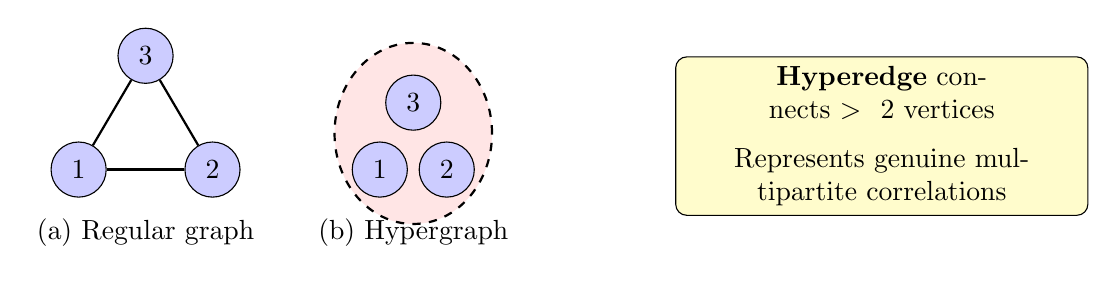
\begin{tikzpicture}[scale=0.85]
		\node[draw, circle, fill=blue!20, minimum size=0.7cm] (1) at (0,0) {1};
		\node[draw, circle, fill=blue!20, minimum size=0.7cm] (2) at (2,0) {2};
		\node[draw, circle, fill=blue!20, minimum size=0.7cm] (3) at (1,1.7) {3};
		\draw[thick] (1) -- (2);
		\draw[thick] (2) -- (3);
		\draw[thick] (3) -- (1);
		\node[below=0.5cm] at (1,0) {(a) Regular graph};

		\node[draw, ellipse, dashed, thick, fill=red!10, minimum width=2cm, minimum height=2.3cm] (h) at (5,0.54) {};
		\node[draw, circle, fill=blue!20, minimum size=0.7cm] (a) at (4.5,0) {1};
		\node[draw, circle, fill=blue!20, minimum size=0.7cm] (b) at (5.5,0) {2};
		\node[draw, circle, fill=blue!20, minimum size=0.7cm] (c) at (5,1.0) {3};
		\node[below=0.5cm] at (5,0) {(b) Hypergraph};

		\node[draw, rounded corners, fill=yellow!20, text width=5cm, align=center] at (12,0.5) {
			\textbf{Hyperedge} connects $>2$ vertices\\[0.2cm]
			Represents genuine multipartite correlations
		};
	\end{tikzpicture}
	\caption{Comparison of regular graphs and hypergraphs. In (a), each edge connects exactly two vertices, representing pairwise correlations. In (b), the dashed ellipse represents a hyperedge connecting three vertices, capturing genuine tripartite entanglement.}
	\label{fig:hypergraph-basic}
\end{figure}

\begin{figure}[htbp]
	\centering
	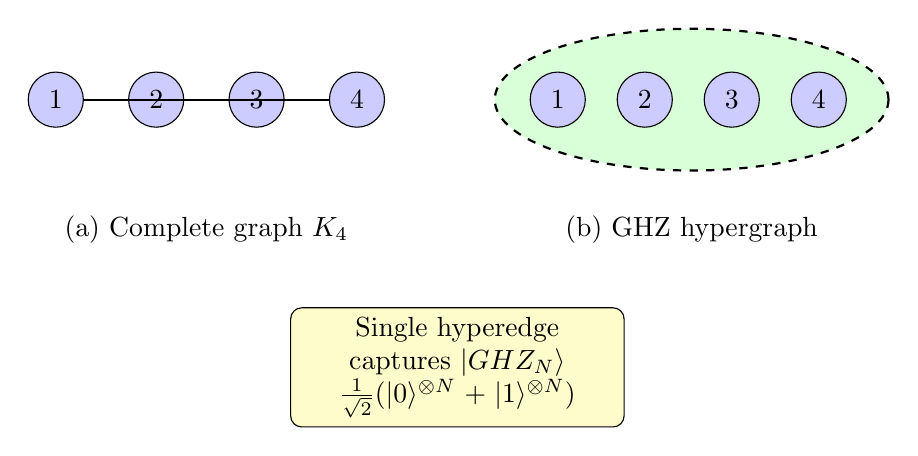
\begin{tikzpicture}[scale=0.85]
		\node[draw, circle, fill=blue!20, minimum size=0.7cm] (1) at (0,0) {1};
		\node[draw, circle, fill=blue!20, minimum size=0.7cm] (2) at (1.5,0) {2};
		\node[draw, circle, fill=blue!20, minimum size=0.7cm] (3) at (3,0) {3};
		\node[draw, circle, fill=blue!20, minimum size=0.7cm] (4) at (4.5,0) {4};
		\draw[thick] (1) -- (2) -- (3) -- (4);
		\draw[thick] (1) -- (3);
		\draw[thick] (2) -- (4);
		\node[below=0.5cm] at (2.25,-1) {(a) Complete graph $K_4$};

		\node[draw, ellipse, dashed, thick, fill=green!15, minimum width=5cm, minimum height=1.8cm] (h) at (9.5,0) {};
		\node[draw, circle, fill=blue!20, minimum size=0.7cm] (n1) at (7.5,0) {1};
		\node[draw, circle, fill=blue!20, minimum size=0.7cm] (n2) at (8.8,0) {2};
		\node[draw, circle, fill=blue!20, minimum size=0.7cm] (n3) at (10.1,0) {3};
		\node[draw, circle, fill=blue!20, minimum size=0.7cm] (n4) at (11.4,0) {4};
		\node[below=0.5cm] at (9.5,-1) {(b) GHZ hypergraph};

		\node[draw, rounded corners, fill=yellow!20, text width=4cm, align=center] at (6,-4) {
			Single hyperedge captures $|GHZ_N\rangle$\\
			$\frac{1}{\sqrt{2}}(|0\rangle^{\otimes N}+|1\rangle^{\otimes N})$
		};
	\end{tikzpicture}
	\caption{GHZ state representation: (a) Complete graph $K_4$ requires many pairwise edges. (b) GHZ hypergraph represents the same state with a single hyperedge connecting all $N$ qubits, capturing the genuine N-partite entanglement.}
	\label{fig:ghz-hypergraph}
\end{figure}

\begin{figure}[htbp]
	\centering
	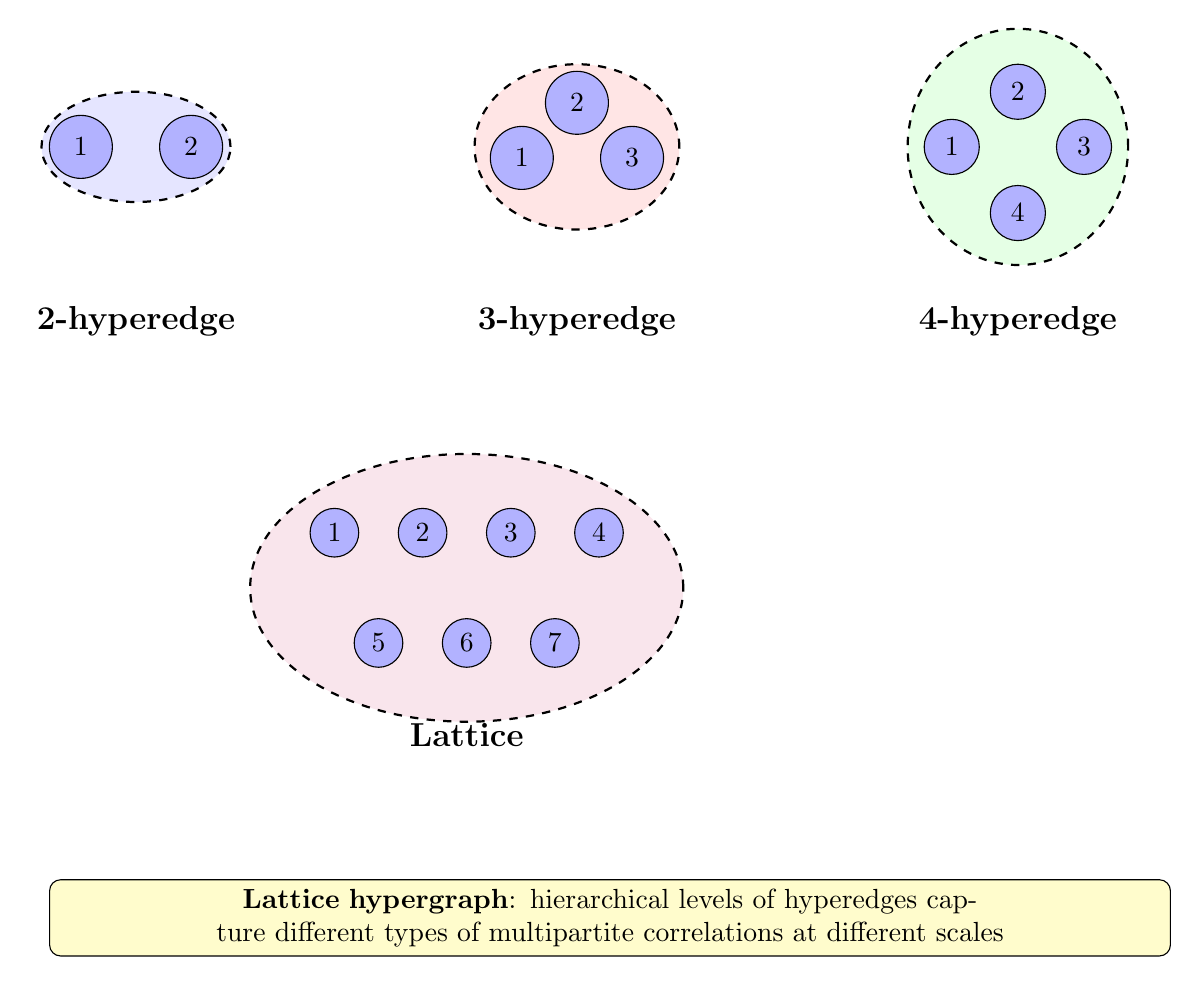
\begin{tikzpicture}[scale=1.4]
		\begin{scope}
			\node[draw, ellipse, dashed, thick, fill=blue!10, minimum width=2.4cm, minimum height=1.4cm] (h2) at (0,0) {};
			\node[draw, circle, fill=blue!30, minimum size=0.8cm] (v1) at (-0.5,0.0) {1};
			\node[draw, circle, fill=blue!30, minimum size=0.8cm] (v2) at (0.5,0.0) {2};
			\node[below=1.9cm] at (0,0) {\large\textbf{2-hyperedge}};
		\end{scope}

		\begin{scope}[xshift=4cm]
			\node[draw, ellipse, dashed, thick, fill=red!10, minimum width=2.6cm, minimum height=2.1cm] (h3) at (0,0) {};
			\node[draw, circle, fill=blue!30, minimum size=0.8cm] (w1) at (-0.5,-0.1) {1};
			\node[draw, circle, fill=blue!30, minimum size=0.8cm] (w2) at (0,0.4) {2};
			\node[draw, circle, fill=blue!30, minimum size=0.8cm] (w3) at (0.5,-0.1) {3};
			\node[below=1.9cm] at (0,0) {\large\textbf{3-hyperedge}};
		\end{scope}

		\begin{scope}[xshift=8cm]
			\node[draw, ellipse, dashed, thick, fill=green!10, minimum width=2.8cm, minimum height=3cm] (h4) at (0,0) {};
			\node[draw, circle, fill=blue!30, minimum size=0.7cm] (x1) at (-0.6,0.0) {1};
			\node[draw, circle, fill=blue!30, minimum size=0.7cm] (x2) at (0,0.5) {2};
			\node[draw, circle, fill=blue!30, minimum size=0.7cm] (x3) at (0.6,0.0) {3};
			\node[draw, circle, fill=blue!30, minimum size=0.7cm] (x4) at (0,-0.6) {4};
			\node[below=1.9cm] at (0,0) {\large\textbf{4-hyperedge}};
		\end{scope}

		\begin{scope}[xshift=3cm, yshift=-4cm]
			\node[draw, ellipse, dashed, thick, fill=purple!10, minimum width=5.5cm, minimum height=3.4cm] (hlattice) at (0,0) {};
			\node[draw, circle, fill=blue!30, minimum size=0.6cm] (y1) at (-1.2,0.5) {1};
			\node[draw, circle, fill=blue!30, minimum size=0.6cm] (y2) at (-0.4,0.5) {2};
			\node[draw, circle, fill=blue!30, minimum size=0.6cm] (y3) at (0.4,0.5) {3};
			\node[draw, circle, fill=blue!30, minimum size=0.6cm] (y4) at (1.2,0.5) {4};
			\node[draw, circle, fill=blue!30, minimum size=0.6cm] (y5) at (-0.8,-0.5) {5};
			\node[draw, circle, fill=blue!30, minimum size=0.6cm] (y6) at (0,-0.5) {6};
			\node[draw, circle, fill=blue!30, minimum size=0.6cm] (y7) at (0.8,-0.5) {7};
			\node[below=1.6cm] at (0,0) {\large\textbf{Lattice}};
		\end{scope}

		\node[draw, rounded corners, fill=yellow!20, text width=14cm, align=center, below=6.5cm] at (4.3,-2) {
			\textbf{Lattice hypergraph}: hierarchical levels of hyperedges capture different types of multipartite correlations at different scales
		};
	\end{tikzpicture}
	\caption{Lattice hypergraph structure showing hierarchical levels. Different hyperedge sizes (2, 3, 4, N) capture correlations at different scales. The full lattice hypergraph combines all levels for complete characterization of multipartite entanglement.}
	\label{fig:lattice-hypergraph}
\end{figure}

\begin{figure}[htbp]
	\centering
	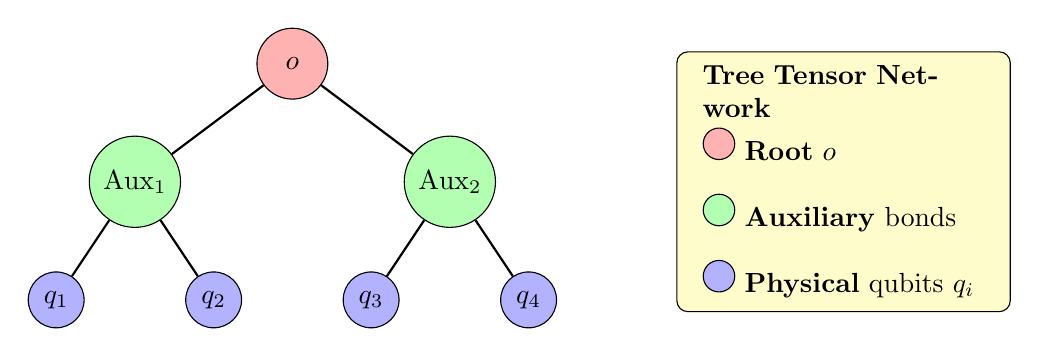
\begin{tikzpicture}[scale=1]
		\begin{scope}
			\node[draw, circle, fill=red!30, minimum size=0.9cm] (root) at (0,3) {$o$};
			\node[draw, circle, fill=green!30, minimum size=0.8cm] (aux1) at (-2,1.5) {Aux$_1$};
			\node[draw, circle, fill=green!30, minimum size=0.8cm] (aux2) at (2,1.5) {Aux$_2$};
			\node[draw, circle, fill=blue!30, minimum size=0.7cm] (q1) at (-3,0) {$q_1$};
			\node[draw, circle, fill=blue!30, minimum size=0.7cm] (q2) at (-1,0) {$q_2$};
			\node[draw, circle, fill=blue!30, minimum size=0.7cm] (q3) at (1,0) {$q_3$};
			\node[draw, circle, fill=blue!30, minimum size=0.7cm] (q4) at (3,0) {$q_4$};

			\draw[thick] (root) -- (aux1);
			\draw[thick] (root) -- (aux2);
			\draw[thick] (aux1) -- (q1);
			\draw[thick] (aux1) -- (q2);
			\draw[thick] (aux2) -- (q3);
			\draw[thick] (aux2) -- (q4);
		\end{scope}

		\begin{scope}[xshift=7cm]
			\node[draw, rounded corners, fill=yellow!20, text width=4cm, align=left] (legend) at (0,1.5) {
				\begin{tabular}{p{3.5cm}}
					\textbf{Tree Tensor Network}                                                                            \\[0.4cm]
					\tikz\node[draw, circle, fill=red!30, inner sep=1pt, minimum size=0.4cm] {}; \textbf{Root} $o$          \\[0.3cm]
					\tikz\node[draw, circle, fill=green!30, inner sep=1pt, minimum size=0.4cm] {}; \textbf{Auxiliary} bonds \\[0.3cm]
					\tikz\node[draw, circle, fill=blue!30, inner sep=1pt, minimum size=0.4cm] {}; \textbf{Physical} qubits $q_i$
				\end{tabular}
			};
		\end{scope}
	\end{tikzpicture}
	\caption{Tree Tensor Network (TTN) representation of multipartite states. Physical qubits ($q_i$) are at the leaf nodes, while auxiliary bonds (Aux$_j$) encode the entanglement geometry. The bond dimension $\chi$ controls the entanglement rank across each cut.}
	\label{fig:tree-tensor-network}
\end{figure}



Tensor network methods, particularly \textbf{tree tensor networks (TTNs)}, provide another visualization framework where the network structure itself represents the entanglement geometry \cite{Hikihara2024}. The TTN structural optimization algorithm can visualize the spatial pattern of spin-singlet pairs in quantum many-body states, with the network structure revealing how entanglement is distributed across the system.

The key insight is that the TTN structure should minimize entanglement entropy at each auxiliary bond, which corresponds to finding the optimal representation of the state's entanglement geometry. This approach has been successfully applied to the rainbow chain model, reproducing the pattern of singlet-pair distribution in the ground state.

\section{Algebraic and Categorical Methods}
\label{sec:algebraic}

Algebraic and categorical methods provide powerful formalisms for reasoning about quantum entanglement through abstract mathematical structures. These approaches, originating from category theory and the theory of compact closed categories, have revolutionized our understanding of quantum processes.

\subsection{ZX Calculus}
\label{sec:zx}

The ZX calculus, developed by Coecke and Duncan \cite{cqm,coecke2008interacting,zx-calculus}, is a diagrammatic calculus for reasoning about quantum processes. It represents quantum states and operations as \textbf{string diagrams} in a compact closed category.

The fundamental objects in the ZX calculus are:
\begin{itemize}
	\item \textbf{Spiders}: Colored nodes (typically red and green) representing certain linear maps. Red spiders (Z spiders) correspond to the computational basis, while green spiders (X spiders) correspond to the Hadamard-transformed basis.
	\item \textbf{Wires}: Lines representing quantum systems (qubits). Input wires enter from the bottom, output wires exit from the top.
	\item \textbf{Standard generators}: The calculus includes identity, Hadamard, and phase gates as basic elements.
\end{itemize}

The key feature of the ZX calculus is the \textbf{spider theorem}: When two spiders of the same color are connected by wires, they can be fused into a single spider. This provides a powerful tool for simplifying quantum circuits and reasoning about entanglement.

For example, the Bell state $|\Phi^+\rangle = \frac{1}{\sqrt{2}}(|00\rangle + |11\rangle)$ is represented as a green spider with two output legs (one for each qubit) connected to a red spider with two input legs, with the appropriate phase angles.

The ZX calculus has proven particularly valuable for visualizing and reasoning about:
\begin{enumerate}
	\item \textbf{Bipartite entanglement}: The Bell states have simple spider representations that make their entanglement structure transparent.
	\item \textbf{Graph state entanglement}: Graph states correspond to certain families of spiders, making the ZX calculus ideal for studying their properties.
	\item \textbf{Quantum circuits}: The calculus provides a visual alternative to circuit diagrams, often revealing structure that is obscured in standard notation.
	\item \textbf{Measurement-based quantum computation}: The one-way quantum computation model has a natural representation in the ZX calculus.
\end{enumerate}

The spider theorem states that when we connect two spiders with any number of wires, the result depends only on the total number of wires, not on how they are connected. This remarkable property encodes the behavior of certain quantum operations and makes the calculus particularly powerful.

A key limitation of the ZX calculus is its primary focus on \textbf{bipartite} entanglement. While it can represent multipartite states, the calculus is most natural for systems with a clear bipartite structure. This limitation motivated the development of the ZW calculus, which explicitly handles multipartite entanglement.

The ZX calculus has been extended in various directions:
\begin{itemize}
	\item \textbf{Completeness}: The calculus is complete for pure qubit quantum mechanics, meaning any identity can be derived from the diagrammatic rules.
	\item \textbf{Generalized ZX}: Extensions to higher-dimensional systems (qudits) and continuous-variable systems.
	\item \textbf{Quantum foundations}: The calculus has been used to provide novel perspectives on quantum foundations and the structure of quantum theory.
\end{itemize}

Graph states, a major class of multipartite entangled states, have a particularly elegant representation in the ZX calculus. A graph state is represented as a collection of green spiders (one for each vertex) connected by yellow Hadamard boxes (which can be decomposed into red-green pairs). This representation makes the stabilizer structure of graph states visually apparent.

The relationship between graph states and ZX diagrams provides:
\begin{itemize}
	\item A visual method for computing stabilizers
	\item Intuitive understanding of local complementation
	\item Tools for studying LC equivalence classes
	\item Connection to the one-way computation model
\end{itemize}

The work of \cite{cqm} provides an in-depth exploration of how the ZX calculus captures the structure of graph states and their entanglement properties, demonstrating how the diagrammatic representation makes manifest the connection between graph structure and quantum correlations.

\begin{figure}[htbp]
	\centering
	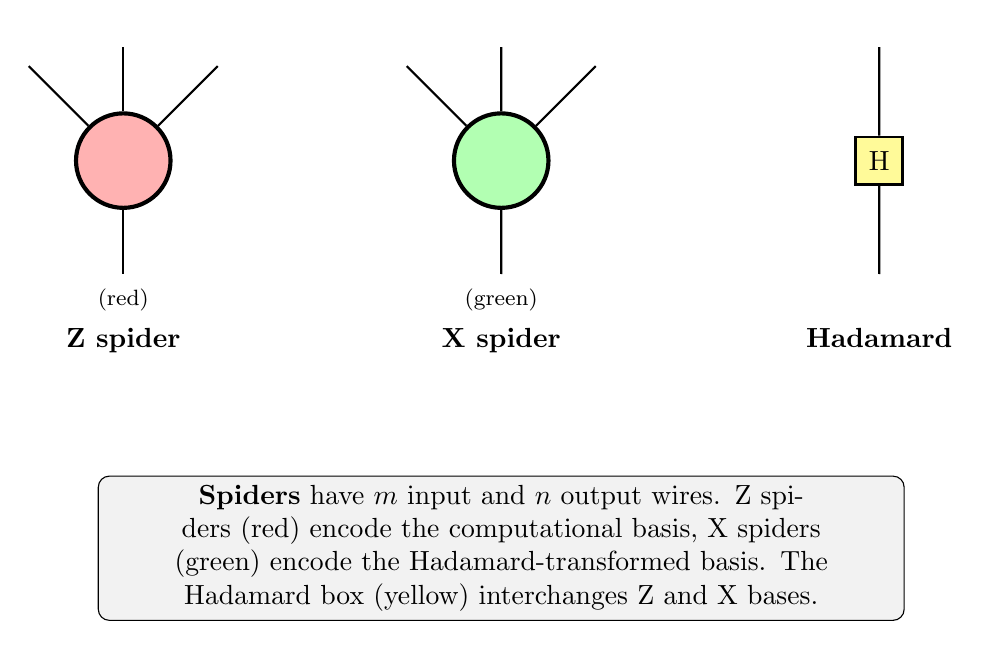
\begin{tikzpicture}[scale=1.2]
		\node[draw, circle, fill=red!30, minimum size=1.2cm, line width=1.5pt] (z) at (0,0) {};
		\draw[thick] (z) -- (0,1.2) node[above] {};
		\draw[thick] (z) -- (0,-1.2) node[below] {};
		\draw[thick] (z) -- (1,1);
		\draw[thick] (z) -- (-1,1);
		\node[below=2.0cm] at (0,0) {\textbf{Z spider}};
		\node[below=1.5cm, font=\footnotesize] at (0,0) {(red)};

		\node[draw, circle, fill=green!30, minimum size=1.2cm, line width=1.5pt] (x) at (4,0) {};
		\draw[thick] (x) -- (4,1.2) node[above] {};
		\draw[thick] (x) -- (4,-1.2) node[below] {};
		\draw[thick] (x) -- (5,1);
		\draw[thick] (x) -- (3,1);
		\node[below=2.0cm] at (4,0) {\textbf{X spider}};
		\node[below=1.5cm, font=\footnotesize] at (4,0) {(green)};

		\node[draw, rectangle, fill=yellow!40, minimum size=0.6cm, line width=1pt] (h) at (8,0) {H};
		\draw[thick] (h) -- (8,1.2) node[above] {};
		\draw[thick] (h) -- (8,-1.2) node[below] {};
		\node[below=2.0cm] at (8,0) {\textbf{Hadamard}};

		\node[draw, rounded corners, fill=gray!10, text width=10cm, align=center, below=1cm] at (4,-2.5) {
			\textbf{Spiders} have $m$ input and $n$ output wires. Z spiders (red) encode the computational basis, X spiders (green) encode the Hadamard-transformed basis. The Hadamard box (yellow) interchanges Z and X bases.
		};
	\end{tikzpicture}
	\caption{Basic elements of the ZX calculus: Z spiders (red, left), X spiders (green, center), and the Hadamard generator (yellow, right). Spiders are the fundamental building blocks representing quantum states and operations.}
	\label{fig:zx-spiders}
\end{figure}

\begin{figure}[htbp]
	\centering
	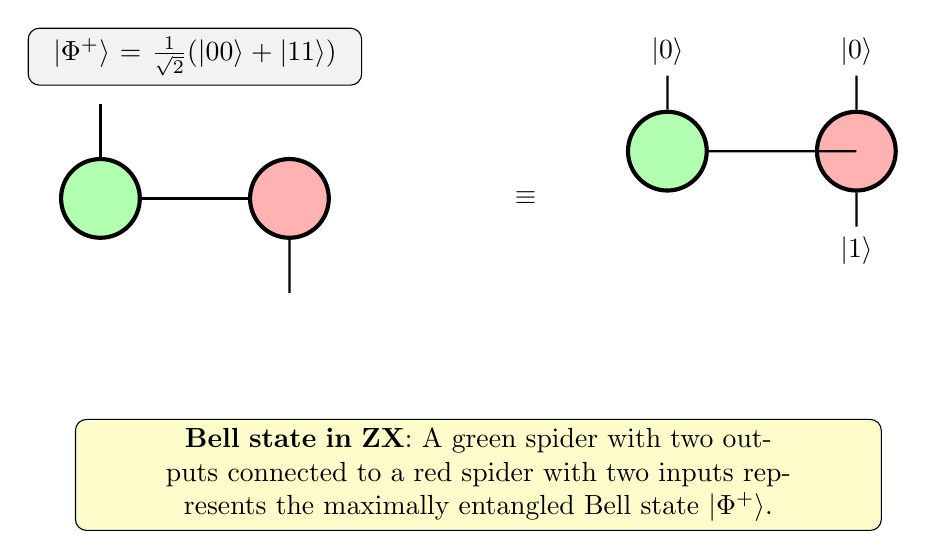
\begin{tikzpicture}[scale=1.2]
		\node[draw, circle, fill=green!30, minimum size=1cm, line width=1.5pt] (g1) at (0,0) {};
		\draw[thick] (g1) -- (0,1) node[above] {};
		\draw[thick] (g1) -- (2,0);

		\node[draw, circle, fill=red!30, minimum size=1cm, line width=1.5pt] (r1) at (2,0) {};
		\draw[thick] (r1) -- (2,-1) node[below] {};

		\node[draw, rounded corners, fill=gray!10, text width=4cm, align=center] at (1,1.5) {
			$|\Phi^+\rangle = \frac{1}{\sqrt{2}}(|00\rangle + |11\rangle)$
		};

		\node at (4.5,0) {$\equiv$};

		\node[draw, circle, fill=green!30, minimum size=1cm, line width=1.5pt] (g2) at (6,0.5) {};
		\node[draw, circle, fill=red!30, minimum size=1cm, line width=1.5pt] (r2) at (8,0.5) {};
		\draw[thick] (g2) -- ++(0,0.8) node[above] {$|0\rangle$};
		\draw[thick] (g2) -- ++(2,0);
		\draw[thick] (r2) -- ++(0,0.8) node[above] {$|0\rangle$};
		\draw[thick] (r2) -- ++(0,-0.8) node[below] {$|1\rangle$};

		\node[draw, rounded corners, fill=yellow!20, text width=10cm, align=center, below=1cm] at (4,-1.5) {
			\textbf{Bell state in ZX}: A green spider with two outputs connected to a red spider with two inputs represents the maximally entangled Bell state $|\Phi^+\rangle$.
		};
	\end{tikzpicture}
	\caption{Bell state $|\Phi^+\rangle$ representation in the ZX calculus. The green spider represents the $|+\rangle$ state in the X basis, and connecting it to the red spider (in Z basis) creates the entangled Bell state.}
	\label{fig:zx-bell-state}
\end{figure}

\begin{figure}[htbp]
	\centering
	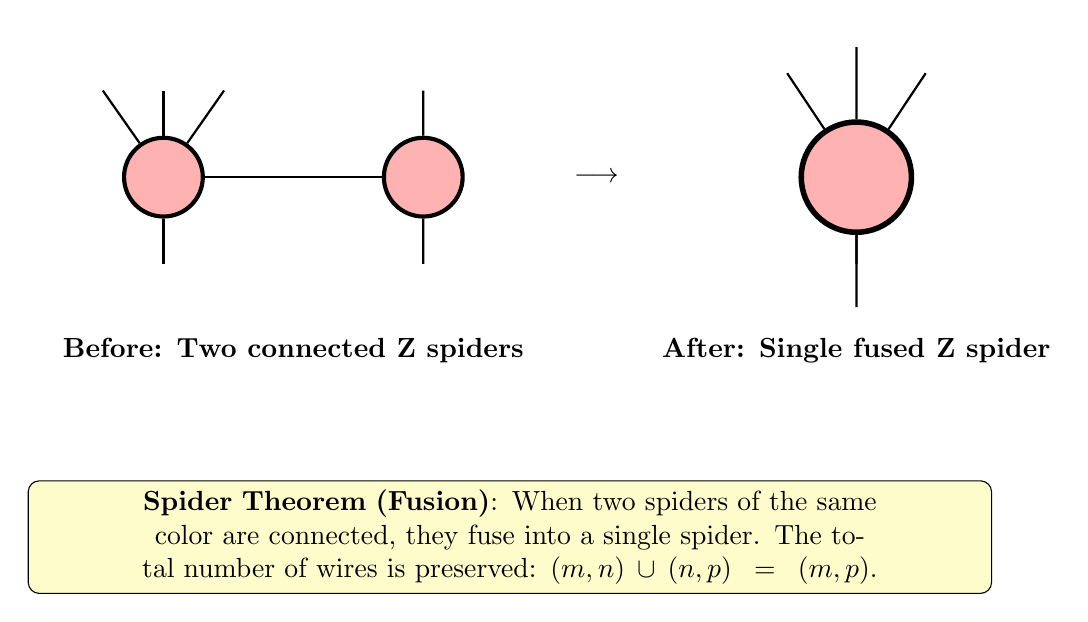
\begin{tikzpicture}[scale=1.1]
		\node[draw, circle, fill=red!30, minimum size=1cm, line width=1.5pt] (r1) at (0,0) {};
		\node[draw, circle, fill=red!30, minimum size=1cm, line width=1.5pt] (r2) at (3,0) {};
		\draw[thick] (r1) -- ++(0,1) node[above] {};
		\draw[thick] (r1) -- ++(-0.7,1);
		\draw[thick] (r1) -- ++(0.7,1);
		\draw[thick] (r1) -- ++(0,-1) node[below] {};
		\draw[thick] (r1) -- (r2);
		\draw[thick] (r2) -- ++(0,1) node[above] {};
		\draw[thick] (r2) -- ++(0,-1) node[below] {};

		\node at (1.5,-2) {\textbf{Before: Two connected Z spiders}};

		\node at (5,0) {$\longrightarrow$};

		\node[draw, circle, fill=red!30, minimum size=1.4cm, line width=2pt] (r3) at (8,0) {};
		\draw[thick] (r3) -- ++(0,1.5) node[above] {};
		\draw[thick] (r3) -- ++(-0.8,1.2);
		\draw[thick] (r3) -- ++(0.8,1.2);
		\draw[thick] (r3) -- ++(0,-1) node[below] {};
		\draw[thick] (r3) -- ++(0,-1.5) node[below] {};

		\node at (8,-2) {\textbf{After: Single fused Z spider}};

		\node[draw, rounded corners, fill=yellow!20, text width=12cm, align=center, below=0cm] at (4,-3.5) {
			\textbf{Spider Theorem (Fusion)}: When two spiders of the same color are connected, they fuse into a single spider. The total number of wires is preserved: $(m,n) \cup (n,p) = (m,p)$.
		};
	\end{tikzpicture}
	\caption{The Spider Theorem in ZX calculus: two connected Z spiders fuse into a single Z spider. This fundamental rule enables simplification of ZX diagrams and reasoning about quantum operations.}
	\label{fig:zx-spider-fusion}
\end{figure}

\begin{figure}[htbp]
	\centering
	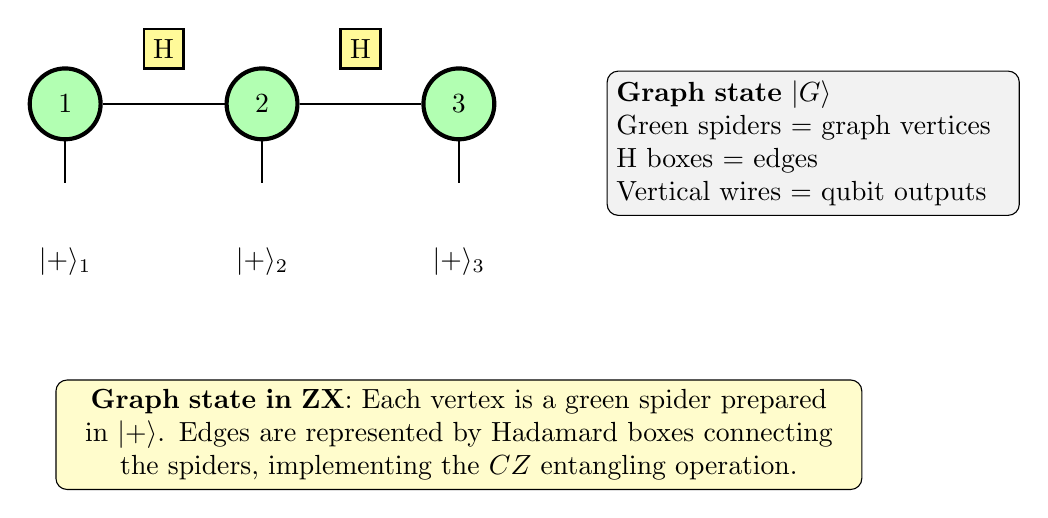
\begin{tikzpicture}[scale=1]
		\node[draw, circle, fill=green!30, minimum size=0.9cm, line width=1.5pt] (g1) at (0,0) {1};
		\node[draw, circle, fill=green!30, minimum size=0.9cm, line width=1.5pt] (g2) at (2.5,0) {2};
		\node[draw, circle, fill=green!30, minimum size=0.9cm, line width=1.5pt] (g3) at (5,0) {3};

		\node[draw, rectangle, fill=yellow!40, minimum size=0.5cm, line width=1pt] (h1) at (1.25,0.7) {H};
		\node[draw, rectangle, fill=yellow!40, minimum size=0.5cm, line width=1pt] (h2) at (3.75,0.7) {H};

		\draw[thick] (g1) -- ++(0,-1) node[below] {};
		\draw[thick] (g2) -- ++(0,-1) node[below] {};
		\draw[thick] (g3) -- ++(0,-1) node[below] {};

		\draw[thick] (g1) -- (g2) -- (g3);

		\node[draw, rounded corners, fill=gray!10, text width=5cm, align=left, xshift=7cm, yshift=-0.5cm] at (2.5,0) {
			\textbf{Graph state $|G\rangle$}\\
			Green spiders = graph vertices\\
			H boxes = edges\\
			Vertical wires = qubit outputs
		};

		\node at (0,-2) {$|+\rangle_1$};
		\node at (2.5,-2) {$|+\rangle_2$};
		\node at (5,-2) {$|+\rangle_3$};

		\node[draw, rounded corners, fill=yellow!20, text width=10cm, align=center, below=0.5cm] at (5.0,-3.0) {
			\textbf{Graph state in ZX}: Each vertex is a green spider prepared in $|+\rangle$. Edges are represented by Hadamard boxes connecting the spiders, implementing the $CZ$ entangling operation.
		};
	\end{tikzpicture}
	\caption{Graph state representation in ZX calculus. Three qubits prepared in $|+\rangle$ (green spiders) are connected by Hadamard boxes (yellow), forming the graph state. The vertical wires represent the physical qubit outputs.}
	\label{fig:zx-graph-state}
\end{figure}

\subsection{ZW Calculus}
\label{sec:zw}

The ZW calculus, introduced by Coecke and Kissinger \cite{zw-calculus,zw-phd}, was specifically designed to address the limitations of the ZX calculus for multipartite entanglement. While ZX excels at representing bipartite structures, ZW provides explicit primitives for representing \textbf{genuine multipartite} entanglement.

The key innovation of the ZW calculus is the introduction of the \textbf{W spider}, which explicitly captures multipartite entanglement. The W spider represents the $N$-partite entangled state:
\begin{equation}
	|W_N\rangle = \frac{1}{\sqrt{N}}(|10\ldots 0\rangle + |01\ldots 0\rangle + \cdots + |00\ldots 1\rangle).
\end{equation}

This state is remarkable because:
\begin{enumerate}
	\item It is genuinely $N$-partite entangled (no bipartition yields a separable state).
	\item It is the unique $N$-qubit state with the property that tracing out any qubit yields the maximally mixed state on the remaining $N-1$ qubits.
	\item It serves as a resource for various quantum protocols.
\end{enumerate}

The ZW calculus thus provides a compositional framework where:
\begin{itemize}
	\item \textbf{Z spiders} (previously represented in ZX as red nodes) represent the computational basis states and are associated with classical bits.
	\item \textbf{W spiders} represent the fundamental multipartite entanglement resource.
	\item \textbf{Composition rules} specify how these primitives combine to form more complex states.
\end{itemize}

The ZW calculus has proven particularly valuable for:
\begin{enumerate}
	\item \textbf{Representing W-type states}: Any state in the W SLOCC class has a natural representation.
	\item \textbf{Understanding GHZ-W conversion}: The calculus makes transparent how GHZ-type and W-type entanglement differ.
	\item \textbf{Studying multipartite entanglement structure}: The W spider provides a primitive for genuine multipartite correlations.
	\item \textbf{Classification of multipartite entanglement}: The calculus provides a framework for distinguishing different entanglement types.
\end{enumerate}

The interplay between Z and W spiders in the calculus mirrors the fundamental distinction between:
\begin{itemize}
	\item \textbf{GHZ-type entanglement}: States like $|\text{GHZ}_N\rangle = \frac{1}{\sqrt{2}}(|0\rangle^{\otimes N} + |1\rangle^{\otimes N})$, which are maximally entangled across any bipartition.
	\item \textbf{W-type entanglement}: States like $|W_N\rangle$, which have distributed entanglement that survives tracing out of any party.
\end{itemize}

This distinction is crucial in multipartite entanglement theory, as GHZ and W states represent inequivalent SLOCC classes for $N \geq 3$.

The ZW calculus extends naturally to the \textbf{ZW* calculus}, which includes additional generators for representing more complex multipartite structures. The calculus has been connected to:
\begin{itemize}
	\item \textbf{Tensor network states}: The diagrammatic representation connects naturally to tensor network notation.
	\item \textbf{Photonic quantum computing}: The calculus provides a natural framework for describing photonic quantum circuits.
	\item \textbf{Quantum foundations}: The calculus has been used to explore the structure of quantum theory from a compositional perspective.
\end{itemize}

The ZX and ZW calculi are not competing but complementary frameworks. The combined ZX-ZW calculus provides a complete toolkit for representing and reasoning about all aspects of multipartite quantum entanglement.

\begin{figure}[htbp]
	\centering
	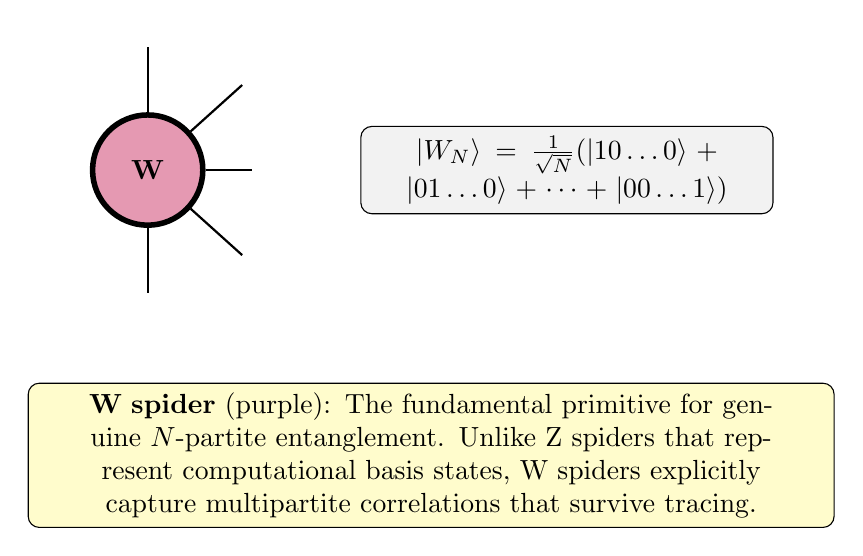
\begin{tikzpicture}[scale=1.2]
		\node[draw, circle, fill=purple!40, minimum size=1.4cm, line width=2pt] (w) at (0,0) {\textbf{W}};
		\draw[thick] (w) -- ++(0,1.3) node[above] {};
		\draw[thick] (w) -- ++(1,0.9);
		\draw[thick] (w) -- ++(1.1,0);
		\draw[thick] (w) -- ++(1,-0.9);
		\draw[thick] (w) -- ++(0,-1.3) node[below] {};

		\node[draw, rounded corners, fill=gray!10, text width=5cm, align=center, right=1.5cm] at (1.0,0) {
			$|W_N\rangle = \frac{1}{\sqrt{N}}(|10\ldots0\rangle + |01\ldots0\rangle + \cdots + |00\ldots1\rangle)$
		};

		\node[draw, rounded corners, fill=yellow!20, text width=10cm, align=center, below=1.5cm] at (3,-1.0) {
			\textbf{W spider} (purple): The fundamental primitive for genuine $N$-partite entanglement. Unlike Z spiders that represent computational basis states, W spiders explicitly capture multipartite correlations that survive tracing.
		};
	\end{tikzpicture}
	\caption{The W spider in ZW calculus represents the N-partite W state. The W spider with $N$ legs encodes the superposition where exactly one qubit is in state $|1\rangle$ and the rest are $|0\rangle$, with all permutations equally weighted.}
	\label{fig:zw-w-spider}
\end{figure}

\begin{figure}[htbp]
	\centering
	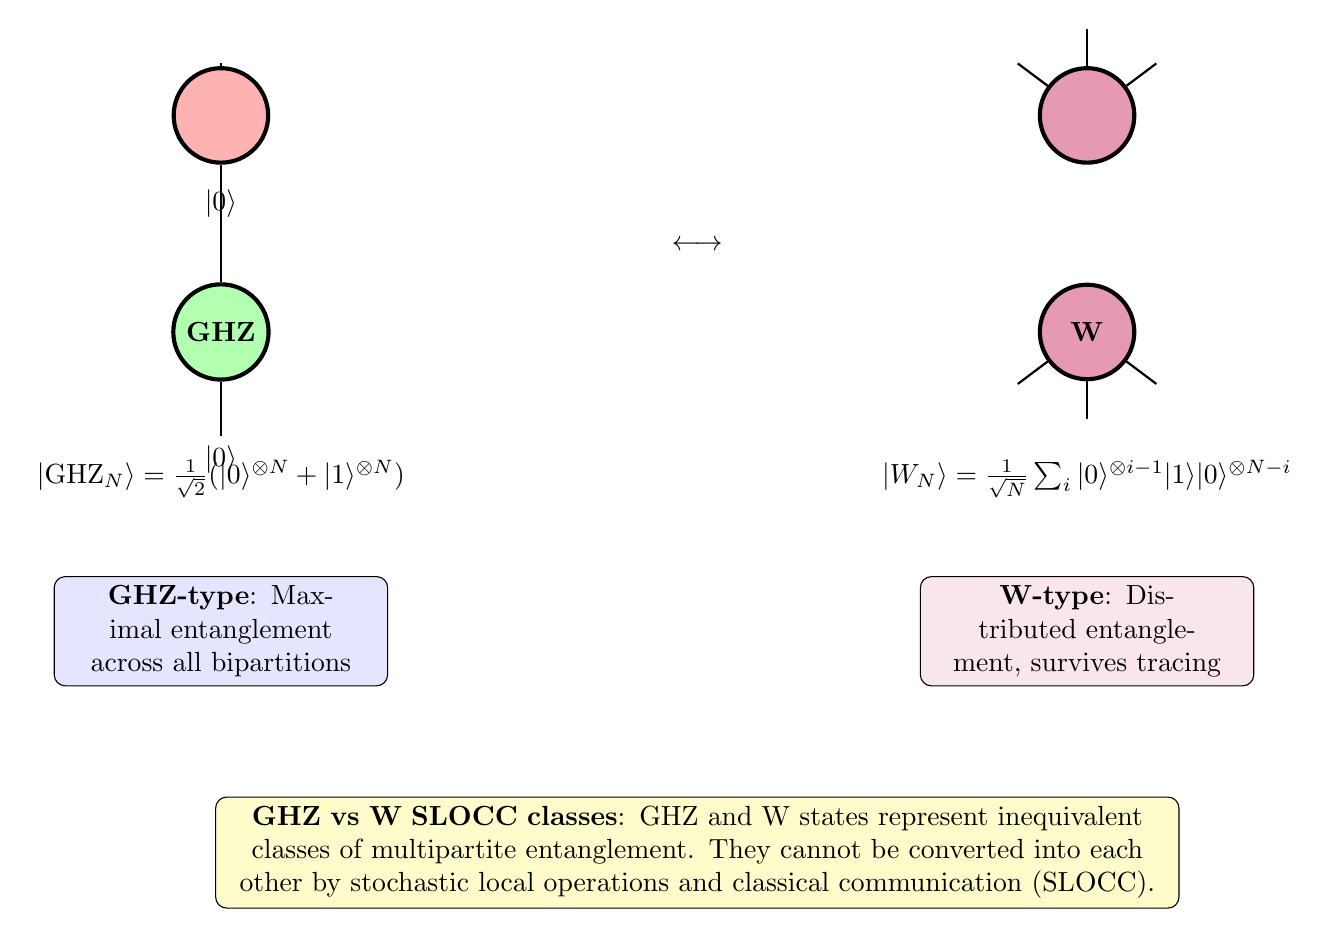
\begin{tikzpicture}[scale=1.1]
		\begin{scope}
			\node[draw, circle, fill=green!30, minimum size=1.2cm, line width=1.5pt] (ghz) at (0,0) {\textbf{GHZ}};
			\draw[thick] (ghz) -- ++(0,1.2) node[above] {$|0\rangle$};
			\draw[thick] (ghz) -- ++(0,-1.2) node[below] {$|0\rangle$};

			\node[draw, circle, fill=red!30, minimum size=1.2cm, line width=1.5pt] (ghz2) at (0,2.5) {};
			\draw[thick] (ghz2) -- ++(0,0.6);
			\draw[thick] (ghz2) -- (ghz);

			\node[below=1.5cm] at (0,0) {$|\text{GHZ}_N\rangle = \frac{1}{\sqrt{2}}(|0\rangle^{\otimes N} + |1\rangle^{\otimes N})$};

			\node[draw, rounded corners, fill=blue!10, text width=4cm, align=center, below=2cm] at (0,-1) {
				\textbf{GHZ-type}: Maximal entanglement across all bipartitions
			};
		\end{scope}

		\node at (5.5,1) {$\longleftrightarrow$};

		\begin{scope}[xshift=10cm]
			\node[draw, circle, fill=purple!40, minimum size=1.2cm, line width=1.5pt] (w1) at (0,0) {\textbf{W}};
			\node[draw, circle, fill=purple!40, minimum size=1.2cm, line width=1.5pt] (w2) at (0,2.5) {};
			\draw[thick] (w1) -- ++(0,-1);
			\draw[thick] (w2) -- ++(0,1);
			\draw[thick] (w1) -- ++(0.8,-0.6);
			\draw[thick] (w1) -- ++(-0.8,-0.6);
			\draw[thick] (w2) -- ++(0.8,0.6);
			\draw[thick] (w2) -- ++(-0.8,0.6);

			\node[below=1.5cm] at (0,0) {$|W_N\rangle = \frac{1}{\sqrt{N}}\sum_i |0\rangle^{\otimes i-1}|1\rangle|0\rangle^{\otimes N-i}$};

			\node[draw, rounded corners, fill=purple!10, text width=4cm, align=center, below=2cm] at (0,-1) {
				\textbf{W-type}: Distributed entanglement, survives tracing
			};
		\end{scope}

		\node[draw, rounded corners, fill=yellow!20, text width=12cm, align=center, below=1.5cm] at (5.5,-4) {
			\textbf{GHZ vs W SLOCC classes}: GHZ and W states represent inequivalent classes of multipartite entanglement. They cannot be converted into each other by stochastic local operations and classical communication (SLOCC).
		};
	\end{tikzpicture}
	\caption{Comparison of GHZ and W states in ZW calculus notation. GHZ states have maximal entanglement across all bipartitions, while W states have distributed entanglement that survives tracing out any single party. These represent distinct SLOCC equivalence classes for $N \geq 3$.}
	\label{fig:zw-ghz-vs-w}
\end{figure}

\begin{figure}[htbp]
	\centering
	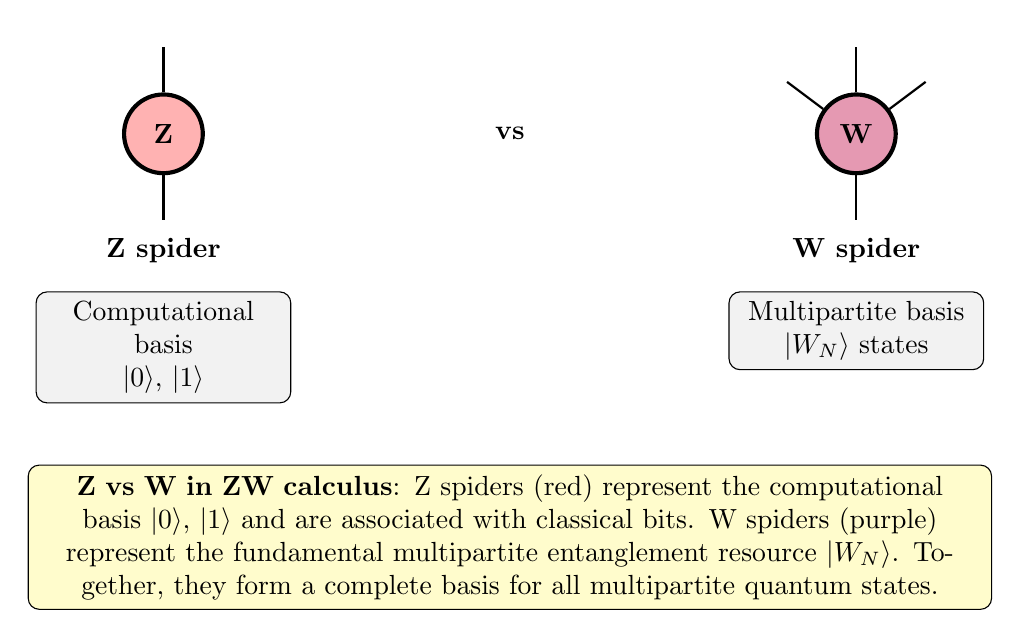
\begin{tikzpicture}[scale=1.1]
		\begin{scope}
			\node[draw, circle, fill=red!30, minimum size=1cm, line width=1.5pt] (z) at (0,0) {\textbf{Z}};
			\draw[thick] (z) -- ++(0,1) node[above] {};
			\draw[thick] (z) -- ++(0,-1) node[below] {};

			\node[below=1.2cm] at (0,0) {\textbf{Z spider}};
			\node[draw, rounded corners, fill=gray!10, text width=3cm, align=center, below=2.0cm] at (0,0) {
				Computational basis\\
				$|0\rangle$, $|1\rangle$
			};
		\end{scope}

		\node at (4,0) {\textbf{vs}};

		\begin{scope}[xshift=8cm]
			\node[draw, circle, fill=purple!40, minimum size=1cm, line width=1.5pt] (w) at (0,0) {\textbf{W}};
			\draw[thick] (w) -- ++(0,1) node[above] {};
			\draw[thick] (w) -- ++(0.8,0.6);
			\draw[thick] (w) -- ++(-0.8,0.6);
			\draw[thick] (w) -- ++(0,-1) node[below] {};

			\node[below=1.2cm] at (0,0) {\textbf{W spider}};
			\node[draw, rounded corners, fill=gray!10, text width=3cm, align=center, below=2.0cm] at (0,0) {
				Multipartite basis\\
				$|W_N\rangle$ states
			};
		\end{scope}

		\node[draw, rounded corners, fill=yellow!20, text width=12cm, align=center, below=2cm] at (4,-2) {
			\textbf{Z vs W in ZW calculus}: Z spiders (red) represent the computational basis $|0\rangle$, $|1\rangle$ and are associated with classical bits. W spiders (purple) represent the fundamental multipartite entanglement resource $|W_N\rangle$. Together, they form a complete basis for all multipartite quantum states.
		};
	\end{tikzpicture}
	\caption{Comparison of Z and W spiders in the ZW calculus. Z spiders encode classical bits in the computational basis, while W spiders provide the primitive for genuine multipartite entanglement. This dual representation enables complete characterization of quantum states.}
	\label{fig:zw-z-vs-w}
\end{figure}

\section{Entanglement Classification and Measures}
\label{sec:classification}

Understanding entanglement requires both classification (distinguishing different types) and quantification (assigning numerical measures). Visualization methods play a crucial role in both aspects.

\subsection{Entanglement Polytopes}
\label{sec:polytopes}

Entanglement polytopes provide a geometric framework for classifying multipartite entanglement by considering the set of possible local measurement statistics. The key idea is to characterize the "entanglement surface" through the possible values of local observables.

Given an $N$-partite quantum state, one can consider the vector of expectation values:
\begin{equation}
	\vec{v}(|\psi\rangle) = (\langle O_1 \rangle, \langle O_2 \rangle, \ldots, \langle O_K \rangle),
\end{equation}
where $\{O_i\}$ are local observables (typically Pauli operators) on each subsystem. For pure states, the set of all possible vectors $\vec{v}$ forms a convex set whose extreme points correspond to product states.

The \textbf{entanglement polytope} is the convex hull of all entanglement vectors achievable by states in a given SLOCC class. Different SLOCC classes correspond to different polytopes, and the position of a state's entanglement vector within its polytope indicates the type and amount of entanglement.

Key features of entanglement polytopes:
\begin{enumerate}
	\item \textbf{Classification}: Different entanglement types correspond to different polytopes.
	\item \textbf{Quantification}: The distance from the polytope boundary indicates how "genuinely" entangled the state is.
	\item \textbf{Testability}: The polytope can be characterized through a finite set of inequalities, making entanglement detection feasible experimentally.
\end{enumerate}

For three qubits, the entanglement polytope is particularly simple: it consists of two tetrahedra corresponding to the GHZ and W SLOCC classes. The three-qubit tangle (a measure of genuine tripartite entanglement) can be related to the volume of the polytope region occupied by the state.

The connection to the Bloch-Norm representation provides a geometric viewpoint where the three-qubit polytope consists of two tetrahedrons, allowing visualization of different entanglement classes and types through Bloch-norms.

The entanglement polytope approach connects to:
\begin{itemize}
	\item \textbf{NPT entanglement detection}: The polytope criteria generalize the Peres-Horodecki criterion to multipartite systems.
	\item \textbf{Quantum marginals}: The problem of determining whether a given set of reduced density matrices is realizable is related to the polytope geometry.
	\item \textbf{Device-independent quantum cryptography}: The polytope framework provides tools for device-independent security analysis.
\end{itemize}

The entanglement simplex provides a complementary viewpoint, where different SLOCC classes occupy distinct regions of a simplex. This connects to the concept of \textbf{entanglement hierarchy} in multipartite systems.

\begin{figure}[htbp]
	\centering
	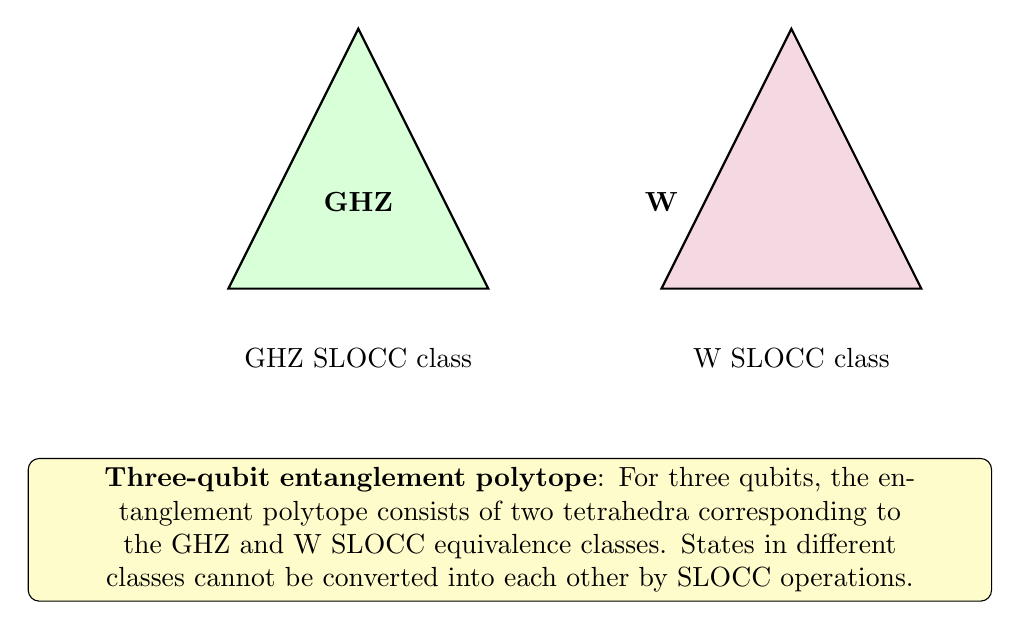
\begin{tikzpicture}[scale=1.1]
		\draw[thick, fill=green!15] (0,0) -- (3,0) -- (1.5,3) -- cycle;
		\node at (1.5,1) {\textbf{GHZ}};

		\draw[thick, fill=purple!15, xshift=5cm] (0,0) -- (3,0) -- (1.5,3) -- cycle;
		\node at (5,1) {\textbf{W}};

		\node at (1.5,-0.8) {GHZ SLOCC class};
		\node at (6.5,-0.8) {W SLOCC class};

		\node[draw, rounded corners, fill=yellow!20, text width=12cm, align=center, below=0.5cm] at (3.25,-1.5) {
			\textbf{Three-qubit entanglement polytope}: For three qubits, the entanglement polytope consists of two tetrahedra corresponding to the GHZ and W SLOCC equivalence classes. States in different classes cannot be converted into each other by SLOCC operations.
		};
	\end{tikzpicture}
	\caption{Three-qubit entanglement polytope showing the two tetrahedra corresponding to GHZ and W SLOCC classes. Each tetrahedron contains all states reachable within that SLOCC class, with product states at the vertices and maximally entangled states in the interior.}
	\label{fig:entanglement-polytope-3qubit}
\end{figure}

\begin{figure}[htbp]
	\centering
	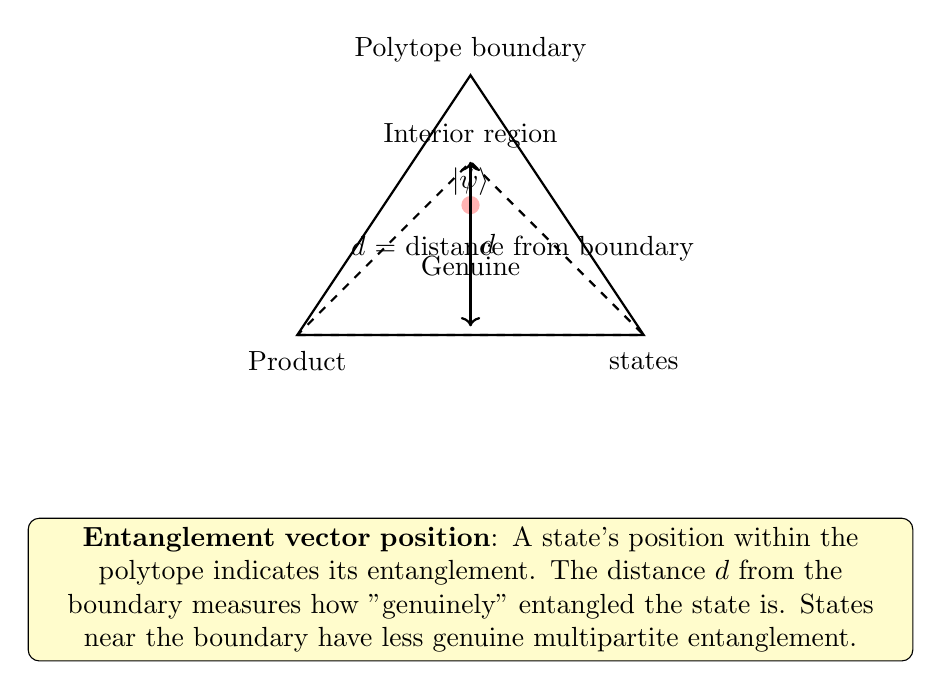
\begin{tikzpicture}[scale=1.1]
		\draw[thick] (0,0) -- (4,0) -- (2,3) -- cycle;
		\draw[dashed, thick] (0,0) -- (4,0) -- (2,2) -- cycle;

		\fill[red!30] (2,1.5) circle (3pt);
		\node[above] at (2,1.5) {$|\psi\rangle$};

		\node at (2,3.3) {Polytope boundary};
		\node at (2,2.3) {Interior region};
		\node at (0,-0.3) {Product};
		\node at (4,-0.3) {states};
		\node at (2,0.8) {Genuine};

		\draw[<->, thick] (2,0.1) -- (2,2) node[midway, right] {$d$};
		\node at (2.6,1) {$d$ = distance from boundary};

		\node[draw, rounded corners, fill=yellow!20, text width=11cm, align=center, below=1cm] at (2,-1.2) {
			\textbf{Entanglement vector position}: A state's position within the polytope indicates its entanglement. The distance $d$ from the boundary measures how "genuinely" entangled the state is. States near the boundary have less genuine multipartite entanglement.
		};
	\end{tikzpicture}
	\caption{Entanglement polytope showing the position of a state $|\psi\rangle$ within the polytope. The distance from the boundary indicates the amount of genuine multipartite entanglement. Extreme points (vertices) correspond to product states, while the interior contains genuinely multipartite entangled states.}
	\label{fig:entanglement-polytope-position}
\end{figure}

\subsection{Entanglement Measures}
\label{sec:measures}

Several entanglement measures have visualizations associated with them:

\textbf{Negativity}: Based on the partial transpose, the negativity $N(\rho) = \frac{||\rho^{T_A}||_1 - 1}{2}$ can be visualized as the "volume" of negative eigenvalues in the partial transpose. For bipartite states, the logarithmic negativity $E_N = \log_2 ||\rho^{T_A}||_1$ provides an additive entanglement measure.

\textbf{Concurrence}: For two qubits, the concurrence $C = \max(0, \lambda_1 - \lambda_2 - \lambda_3 - \lambda_4)$ can be visualized as the "length" of the longest chord in the ellipse of the reduced density matrix in the Bloch representation.

\textbf{Tangle}: The three-qubit tangle $\tau = C_{A(BC)}^2 - C_{AB}^2 - C_{AC}^2$ measures genuine tripartite entanglement and can be visualized as the "area" of a triangle formed by the three concurrences.

Recent work on \textbf{geometric measures of entanglement} provides visualization through distances in Hilbert space:
\begin{itemize}
	\item \textbf{Geometric measure}: $E_G(|\psi\rangle) = \min_{|\phi\rangle \in \text{SEP}} |||\psi\rangle - |\phi\rangle||^2$, where the minimum is over separable states.
	\item \textbf{Triangle measure}: For three qubits, the squared tangle equals the area of a triangle formed by the three one-to-other entropies.
	\item \textbf{Tetrahedron measure}: For four qubits, a tetrahedron measure provides a connection between multipartite entanglement and the hypervolume of geometric simplices.
\end{itemize}

The work demonstrates that the area of a triangle formed by one-to-other entropies can measure three-qubit GME, with squared area proportional to the tangle. For four qubits, the four-qubit entropic fill relates to the hypervolume of a tetrahedron whose face areas are given by the one-to-other entropies.

The \textbf{entanglement distance} (ED) \cite{EntanglementDistance} provides a measure based on the Fubini-Study metric. For a state $|s\rangle$, the single-qubit ED is defined as:
\begin{equation}
	E_\mu(|s\rangle) = 1 - \sum_{j=x,y,z} |\langle s|\sigma_j^\mu|s\rangle|^2,
\end{equation}
which ranges from 0 (pure product state) to 1 (maximally mixed). The total entanglement is the sum over all qubits. This measure has been applied to study entanglement in pseudo-graph states, showing that vertex degree distribution determines entanglement properties.

The entanglement distance approach reveals that:
\begin{itemize}
	\item Local connectivity of the underlying graph determines the entanglement.
	\item The measure is invariant under vertex relabeling, highlighting its topological character.
	\item It depends only on the total degree of each vertex, not on the distinction between incoming and outgoing edges.
\end{itemize}

Recent work \cite{SpanningGraphs2025} introduces graphical representations based on \textbf{minimal spanning graphs} that allow identification of genuine multipartite entanglement in hybrid quantum circuits. This approach provides a framework for understanding how measurements and unitary evolution work together to produce entanglement spreading.

The \textbf{tangle} has a clear geometric interpretation in the three-qubit case: $\tau = C_{A(BC)}^2 - C_{AB}^2 - C_{AC}^2$, which can be visualized as the "excess" entanglement beyond what can be explained by pairwise correlations. The relationship between tangle and the Bloch-norm allows deriving bounds that depend on the entanglement class.

For higher-partite systems, the \textbf{hierarchy of monogamy relations} provides visualizations through inequalities relating entanglement across different bipartitions. The Coffman-Kundu-Wootters (CKW) inequality for three qubits was one of the first examples:
\begin{equation}
	C_{AB}^2 + C_{AC}^2 \leq C_{A(BC)}^2,
\end{equation}
which can be visualized as a triangle inequality where the "full" entanglement $C_{A(BC)}$ is the hypotenuse.

\begin{figure}[htbp]
	\centering
	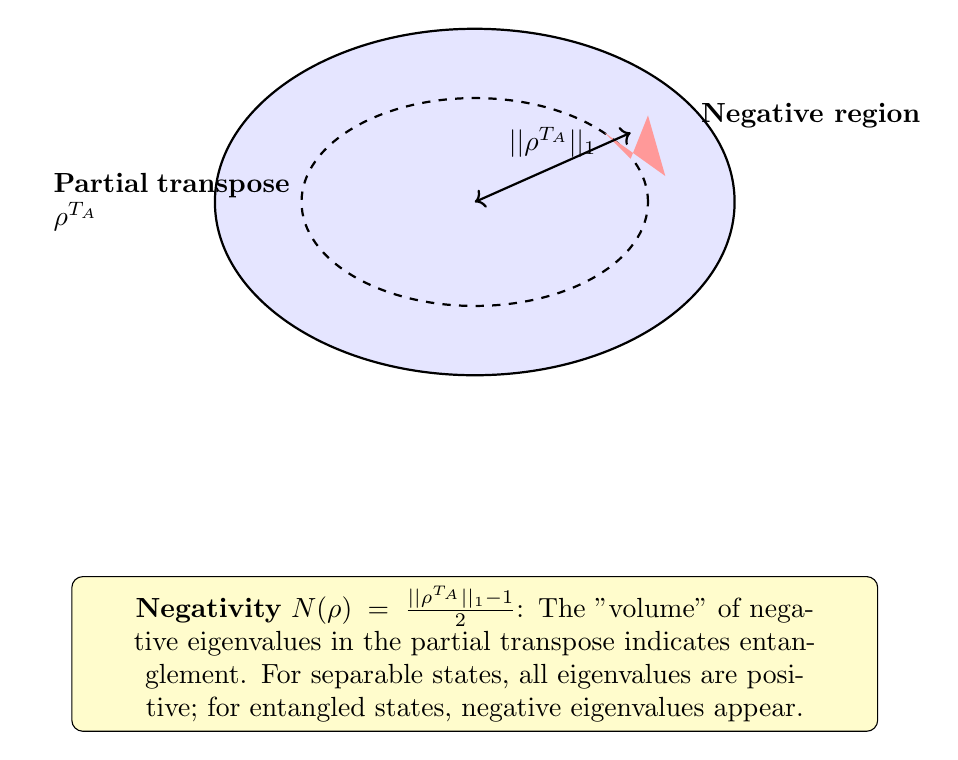
\begin{tikzpicture}[scale=1.1]
		\draw[thick, fill=blue!10] (0,0) ellipse (3cm and 2cm);

		\draw[thick, dashed] (0,0) ellipse (2cm and 1.2cm);

		\fill[red!40] (1.5,0.8) -- (2.2,0.3) -- (2.0,1.0) -- (1.8,0.5) -- cycle;

		\node at (-3.5,0) {
			\begin{tabular}{p{3cm}}
				\textbf{Partial transpose} \\
				$\rho^{T_A}$
			\end{tabular}
		};

		\node[right] at (2.5,1) {\textbf{Negative region}};

		\draw[<->, thick] (0,0) -- (1.8,0.8) node[midway, above] {$||\rho^{T_A}||_1$};

		\node[draw, rounded corners, fill=yellow!20, text width=10cm, align=center, below=2cm] at (0,-2.5) {
			\textbf{Negativity} $N(\rho) = \frac{||\rho^{T_A}||_1 - 1}{2}$: The "volume" of negative eigenvalues in the partial transpose indicates entanglement. For separable states, all eigenvalues are positive; for entangled states, negative eigenvalues appear.
		};
	\end{tikzpicture}
	\caption{Negativity visualization: the partial transpose $\rho^{T_A}$ of an entangled state has negative eigenvalues (shown in red). The negativity $N(\rho)$ measures the total "volume" of these negative regions, providing a quantifier of bipartite entanglement.}
	\label{fig:negativity-visualization}
\end{figure}

\begin{figure}[htbp]
	\centering
	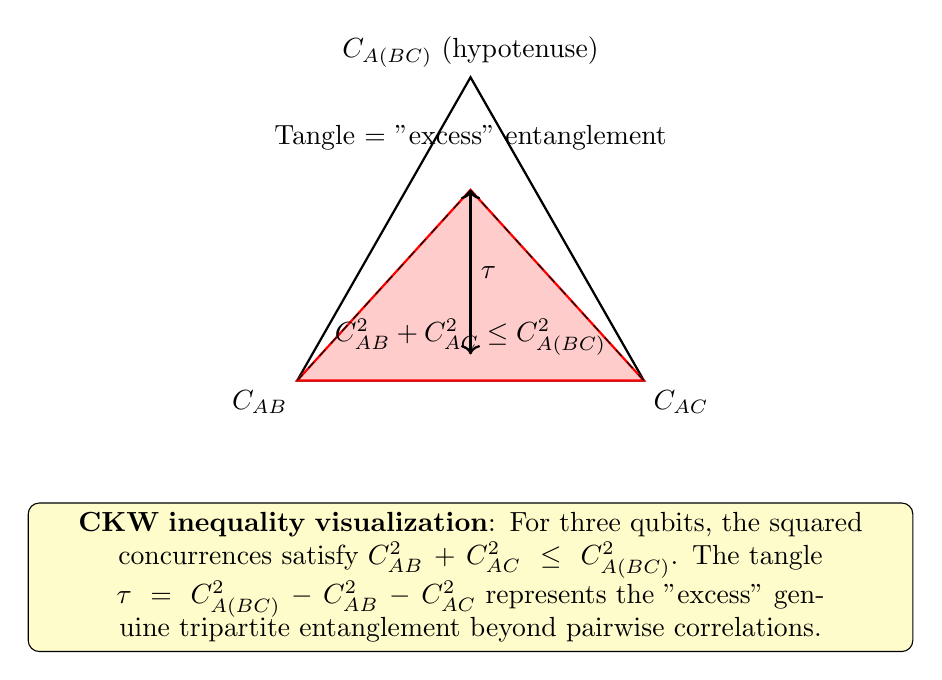
\begin{tikzpicture}[scale=1.1]
		\draw[thick] (0,0) -- (4,0) -- (2,3.5) -- cycle;

		\draw[thick, red, fill=red!20] (0,0) -- (4,0) -- (2,2.2) -- cycle;

		\node at (2,0.5) {$C_{AB}^2 + C_{AC}^2 \leq C_{A(BC)}^2$};

		\node[below left] at (0,0) {$C_{AB}$};
		\node[below right] at (4,0) {$C_{AC}$};
		\node[above] at (2,3.5) {$C_{A(BC)}$ (hypotenuse)};

		\draw[<->, thick] (2,0.3) -- (2,2.2) node[midway, right] {$\tau$};

		\node at (2,2.8) {Tangle = "excess" entanglement};

		\draw[dashed] (4,0) -- (2,2.2);
		\draw[dashed] (0,0) -- (2,2.2);

		\node[draw, rounded corners, fill=yellow!20, text width=11cm, align=center, below=1cm] at (2,-0.5) {
			\textbf{CKW inequality visualization}: For three qubits, the squared concurrences satisfy $C_{AB}^2 + C_{AC}^2 \leq C_{A(BC)}^2$. The tangle $\tau = C_{A(BC)}^2 - C_{AB}^2 - C_{AC}^2$ represents the "excess" genuine tripartite entanglement beyond pairwise correlations.
		};
	\end{tikzpicture}
	\caption{Coffman-Kundu-Wootters (CKW) inequality visualization for three qubits. The triangle inequality shows that the squared entanglement $C_{A(BC)}^2$ (hypotenuse) must be at least as large as the sum of squared pairwise entanglements $C_{AB}^2 + C_{AC}^2$. The tangle $\tau$ represents the genuine tripartite entanglement not captured by pairwise measures.}
	\label{fig:ckw-inequality}
\end{figure}

\begin{figure}[htbp]
	\centering
	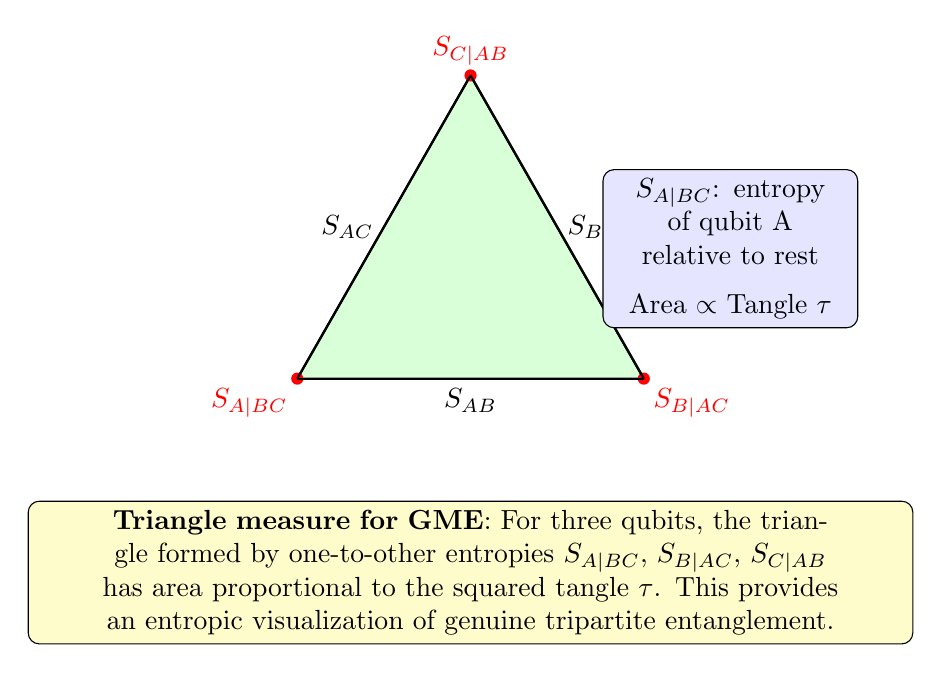
\begin{tikzpicture}[scale=1.1]
		\coordinate (A) at (0,0);
		\coordinate (B) at (4,0);
		\coordinate (C) at (2,3.5);

		\draw[thick, fill=green!15] (A) -- (B) -- (C) -- cycle;

		\fill[red] (A) circle (2pt) node[below left] {$S_{A|BC}$};
		\fill[red] (B) circle (2pt) node[below right] {$S_{B|AC}$};
		\fill[red] (C) circle (2pt) node[above] {$S_{C|AB}$};

		\draw[thick] (A) -- (B) node[midway, below] {$S_{AB}$};
		\draw[thick] (B) -- (C) node[midway, right] {$S_{BC}$};
		\draw[thick] (C) -- (A) node[midway, left] {$S_{AC}$};

		\node[draw, rounded corners, fill=blue!10, text width=3cm, align=center] at (5,1.5) {
			$S_{A|BC}$: entropy of qubit A relative to rest\\
			\vspace{0.2cm}
			Area $\propto$ Tangle $\tau$
		};

		\node[draw, rounded corners, fill=yellow!20, text width=11cm, align=center, below=1cm] at (2,-0.5) {
			\textbf{Triangle measure for GME}: For three qubits, the triangle formed by one-to-other entropies $S_{A|BC}$, $S_{B|AC}$, $S_{C|AB}$ has area proportional to the squared tangle $\tau$. This provides an entropic visualization of genuine tripartite entanglement.
		};
	\end{tikzpicture}
	\caption{Triangle measure for three-qubit genuine multipartite entanglement. The one-to-other entropies $S_{A|BC}$, $S_{B|AC}$, $S_{C|AB}$ form a triangle whose area is proportional to the squared tangle $\tau$. This connects geometric and entropic measures of entanglement.}
	\label{fig:triangle-measure}
\end{figure}

\section{Specialized State Classes}
\label{sec:specialized}

Certain families of quantum states have special structure that enables tailored visualization approaches. This section covers the most important such families.

\subsection{Symmetric States}
\label{sec:symmetric}

Symmetric states are invariant under permutation of all qubits: $P_\pi |\psi\rangle = |\psi\rangle$ for all permutations $\pi$. These states have attracted significant attention because:
\begin{enumerate}
	\item They are described by only $2N$ real parameters (versus $2^{N+1} - 2$ for general states).
	\item They exhibit interesting multipartite entanglement despite their symmetry.
	\item They arise naturally in systems of identical particles and collective spin systems.
	\item They are easier to characterize and visualize.
\end{enumerate}

The Dicke basis provides an important representation for symmetric states. The $N$-qubit Dicke state with excitation number $k$, denoted $|D_N^k\rangle$, is the uniform superposition of all computational basis states with exactly $k$ ones:
\label{sec:dicke}
\begin{equation}
	|D_N^k\rangle = \frac{1}{\sqrt{\binom{N}{k}}} \sum_{\text{perm}} |i_1 i_2 \ldots i_N\rangle,
\end{equation}
where the sum is over all permutations with exactly $k$ ones.

The $k=1$ case gives the $W$ state: $|W_N\rangle = |D_N^1\rangle$. The $k=N/2$ case (for even $N$) gives the symmetric state with maximal total spin.

Majorana representation provides the natural visualization framework for symmetric states (see \cref{sec:majorana}). The $N$ points of the Majorana constellation provide a complete description of the state's entanglement properties.

For symmetric states, the Majorana constellation provides:
\begin{itemize}
	\item A complete classification: Different constellation geometries correspond to different SLOCC classes.
	\item Visual intuition: The distribution of points relates to entanglement type.
	\item Connection to stability: The sensitivity of the constellation to perturbations indicates stability of the entanglement.
\end{itemize}

The study of highly symmetric multipartite states \cite{burchardt2021} shows how group theory can construct genuinely entangled states with desired symmetry properties. These states resemble Dicke states but have interactions occurring only between specific subsystems related by group actions.

The entanglement properties of symmetric states include:
\begin{itemize}
	\item \textbf{Dicke states} exhibit genuine $N$-partite entanglement for $k \neq 0, N$.
	\item \textbf{Permutationally invariant states} can be characterized by their "entanglement spectrum" --- the set of eigenvalues of reduced density matrices.
	\item \textbf{Classification}: Symmetric states can be completely classified using the Majorana representation, with the number and arrangement of degenerate points indicating entanglement type.
\end{itemize}

The connection between Dicke states and entropy cones demonstrates that all possible Dicke state entropy vectors emerge symmetrized. A min-cut protocol on star graphs can realize the entropy vectors, connecting hypergraph structure to entanglement entropy.

The geometric measure of entanglement for symmetric states can be computed by considering the minimum distance to the set of separable symmetric states. This has been studied extensively for Dicke states, particularly in the context of quantum metrology where symmetric states can achieve the Heisenberg limit.

Stabilizer formalism provides another tool for symmetric states: the Dicke states are stabilizer states with particular stabilizer groups. The representation of stabilizer states in the Dicke basis reveals interesting combinatorial properties.

Symmetric states are also important in quantum optics and many-body physics, where they arise naturally as states of collective spin systems. The Holstein-Primakoff representation connects symmetric states to bosonic systems, enabling visualization through phase space methods.

Stabilizer states are a broad class of quantum states that can be characterized by their stabilizer groups. A stabilizer state $|\psi\rangle$ is uniquely defined by a set of $N$ commuting Pauli operators $\{g_1, \ldots, g_N\}$ such that $g_i |\psi\rangle = |\psi\rangle$ for all $i$. The stabilizer group $\mathcal{S} = \langle g_1, \ldots, g_N \rangle$ contains $2^N$ elements.

Graph states (see \cref{sec:graph-states}) form a prominent subclass of stabilizer states that admit a graphical representation. However, not all stabilizer states are LC-equivalent to graph states. For $N \geq 8$, there exist stabilizer states that cannot be represented as graph states.

The visualization of stabilizer states includes:
\begin{enumerate}
	\item \textbf{Stabilizer diagrams}: Representing the stabilizer generators as nodes in a graph, with edges indicating commutation relations.
	\item \textbf{Pauli weight distribution}: The distribution of Pauli weights (number of non-identity Pauli operators) in the stabilizer group provides information about entanglement structure \cite{GraphStateVis}.
	\item \textbf{Entanglement structure visualization}: Using the methods of entangled graphs to represent the entanglement structure revealed by the stabilizer.
\end{enumerate}

The Clifford group plays an important role in stabilizer states: it maps stabilizer states to stabilizer states. The action of Clifford operations can be visualized through their effect on the stabilizer graph.

Stabilizer states have been classified up to local Clifford equivalence for small numbers of qubits:
\begin{itemize}
	\item \textbf{1 qubit}: 2 states (trivial).
	\item \textbf{2 qubits}: 2 states (product state and Bell state).
	\item \textbf{3 qubits}: 2 SLOCC classes (GHZ and W).
	\item \textbf{4 qubits}: 9 SLOCC classes, with many more LU classes.
	\item \textbf{Higher N}: The number of classes grows rapidly; complete classification remains an open problem.
\end{itemize}

The connection between stabilizer states and classical codes provides another visualization perspective:
\begin{itemize}
	\item \textbf{Graph codes}: Stabilizer codes can be represented by graphs, connecting error correction to entanglement.
	\item \textbf{k-UNI states}: States with maximum entanglement across all bipartitions of size $k$ can be constructed from classical codes \cite{Raissi2021}.
	\item \textbf{AME states}: Absolutely maximally entangled states represent the strongest form of multipartite entanglement.
\end{itemize}

The study of \textbf{symmetries in stabilizer states} \cite{Englbrecht2020} reveals how the entanglement structure is related to the symmetry group. States with high symmetry often have special entanglement properties.

The \textbf{local information access} in graph states relates to the graph connectivity: the amount of entanglement that can be extracted between different subsets of qubits is determined by the graph structure.

The graphical description by Elliott, Eastin, and Caves provides a comprehensive framework for understanding how Pauli measurements and Clifford operations affect stabilizer states, with the graphical representation making manifest the connection between the stabilizer formalism and entanglement structure.

Recent work on \textbf{transformations of stabilizer states in quantum networks} demonstrates how to decompose stabilizer states into tensor products of indecomposable states from the entanglement generating set (EGS), which is finite up to 10 qubits.

The reachability graphs in stabilizer states connect to entropy vectors: given a stabilizer state, the reachability graph captures which reduced density matrices can be reached through partial tracing. This provides a visualization of the entanglement structure.

Dicke states have a natural representation in the stabilizer formalism. The $|D_N^k\rangle$ state has a stabilizer group with interesting properties:
\begin{itemize}
	\item The logical operators correspond to certain strings of Pauli operators.
	\item The codespace properties relate to error correction.
	\item The connection to symmetric informationally complete (SIC) POVMs provides another perspective.
\end{itemize}

The matrix product state (MPS) representation of Dicke states provides an exact canonical representation with minimal bond dimension $\chi = k+1$. This representation can be used to formulate quantum circuits for deterministic preparation of Dicke states.

The MPS representation connects naturally to tensor network visualization, where:
\begin{itemize}
	\item Each tensor corresponds to a local Hilbert space.
	\item Contraction corresponds to entanglement structure.
	\item Bond dimension corresponds to entanglement rank.
\end{itemize}

The entropy cone for Dicke states demonstrates that all $|D_N^k\rangle$ entropy vectors emerge symmetrized, and the min-cut protocol on star graphs realizes these entropy vectors. This provides a connection between discrete graph structure and continuous entanglement entropy.

Recent work on \textbf{quantum circuits for Dicke states} provides efficient circuits of depth O(n) for preparing N-qubit Dicke states, making them experimentally relevant for NISQ-era quantum processors.

W-states and GHZ-states represent two fundamentally different types of multipartite entanglement that cannot be converted into each other using SLOCC operations. Their visualization:

\begin{enumerate}
	\item \textbf{W-states}: $|W_N\rangle$ have all possible pairwise entanglements equal, with reduced states always maximally mixed. The Majorana constellation has $N-1$ points at the north pole and one at the south pole.

	\item \textbf{GHZ-states}: $|\text{GHZ}_N\rangle$ have maximal entanglement across any bipartition but are separable when tracing out any party. The Majorana constellation has two points at opposite poles.
\end{enumerate}

The conversion between these types requires operations that go beyond SLOCC, highlighting their fundamental difference in entanglement structure.

Measuremnt-Based Quantum Computation (MBQC) uses graph states as the primary resource. The visualization of MBQC protocols:
\begin{itemize}
	\item The \textbf{quantum circuit} is replaced by a \textbf{measurement pattern} on a graph state.
	\item The order of measurements determines the computation.
	\item The underlying graph structure encodes the parallelism and dependencies in the computation.
\end{itemize}

This provides a powerful visual paradigm for quantum computation where the "program" is a graph and "data" are measurement outcomes.

Quantum networks use graph states to establish entanglement between distant nodes:
\begin{itemize}
	\item \textbf{Graph state distribution}: Creating graph states across a network.
	\item \textbf{Quantum routing}: Using graph transformations to route entanglement.
	\item \textbf{Network topology}: The network structure determines achievable entanglement configurations.
\end{itemize}

The visualization of entanglement in quantum networks thus naturally uses graph-based methods.

The recent work on \textbf{entanglement-assisted non-local optical interferometry} in quantum networks demonstrates experimental progress in distributing multipartite entanglement across nodes. Such experiments rely on the visualization and characterization of entanglement structure.

Continuous-variable (CV) systems provide another arena for entanglement visualization. The phase space methods mentioned in \cref{sec:phase-space} become particularly natural for CV systems:
\begin{itemize}
	\item Wigner functions provide quasi-probability distributions.
	\item Negativity in the Wigner function indicates non-classicality.
	\item Gaussian vs. non-Gaussian entanglement can be distinguished through phase space properties.
\end{itemize}

Recent work on \textbf{continuous-variable fault-tolerant quantum computation} under general noise demonstrates the importance of understanding entanglement in CV systems for practical quantum computing.

Tensor network visualizations provide a powerful framework for understanding entanglement in many-body systems:
\begin{itemize}
	\item The network structure encodes the entanglement geometry.
	\item Bond dimensions correspond to entanglement rank across cuts.
	\item Different network architectures (MPS, PEPS, TTN, MERA) capture different entanglement structures.
\end{itemize}

The TTN structural optimization algorithm \cite{Hikihara2024} demonstrates how optimal network structure can reveal entanglement geometry in quantum many-body systems. This approach can:
\begin{itemize}
	\item Visualize the spatial pattern of spin-singlet pairs.
	\item Reproduce the pattern of singlet-pair distribution in the ground state.
	\item Show that the algorithm minimizes truncation error while revealing entanglement structure.
\end{itemize}

The rainbow chain model provides an excellent test case: its ground state is approximately a product state of singlet pairs between spins separated by various distances. The TTN optimization reveals this structure naturally.

MERA (Multiscale Entanglement Renormalization Ansatz) provides another visualization framework where the hierarchical structure of the network reflects the entanglement scaling in critical systems.

Quantum error correction codes provide a visualization of entanglement through the stabilizer formalism:
\begin{itemize}
	\item The code space is the simultaneous +1 eigenspace of the stabilizer.
	\item Logical operators encode non-local entanglement.
	\item The error-correcting properties relate to the distance of the code, which is a graph-theoretic property.
\end{itemize}

The connection to graph codes shows how error correction and entanglement are two sides of the same coin.

Entanglement entropy provides a fundamental quantity for characterizing many-body entanglement:
\begin{itemize}
	\item The area law for gapped systems.
	\item Logarithmic corrections at criticality.
	\item The bipartite entanglement spectrum as a fingerprint of entanglement structure.
\end{itemize}

The visualization of entanglement entropy through \textbf{entropy vectors} and \textbf{entropy cones} provides a geometric framework for understanding multipartite entanglement structure.

Renyi entropies provide a family of entanglement measures that can be visualized through their $\alpha$-dependence. Different $\alpha$ values probe different aspects of the entanglement spectrum.

The relationship between entanglement and measurement-induced phase transitions provides a recent frontier:
\begin{itemize}
	\item Hybrid quantum circuits with measurements show entanglement spreading.
	\item Minimal spanning graphs can indicate GME.
	\item The entanglement transition can be visualized through graph properties.
\end{itemize}

The work on \textbf{measurement-induced entanglement transitions} \cite{SpanningGraphs2025} demonstrates how graphical methods can reveal the structure of entanglement in complex quantum dynamics.

Quantum machine learning provides new frontiers for entanglement visualization:
\begin{itemize}
	\item Variational ansätze (PQCs, QAOA) have entanglement structure that can be visualized.
	\item Expressibility and entanglement capabilities can be analyzed graphically.
	\item Tensor network visualizations can help understandbarrier landscapes.
\end{itemize}

This remains an active area of research where visualization methods are crucial for understanding the power of quantum learning models.

Quantum foundations provides another perspective on entanglement visualization:
\begin{itemize}
	\item The structure of quantum theory can be explored through compositional graphical methods.
	\item The ZX/ZW calculi provide tools for understanding what makes quantum mechanics distinctive.
	\item The resource theories of entanglement provide operational meaning to visualization.
\end{itemize}

This perspective connects entanglement visualization to fundamental questions about the nature of quantum mechanics.

Looking forward, several frontiers remain active areas of research:

\begin{enumerate}
	\item \textbf{Higher-dimensional systems}: Extending visualization methods beyond to qud qubitsits and continuous-variable systems.
	\item \textbf{Dynamics}: Visualizing entanglement generation and propagation in real-time.
	\item \textbf{Open quantum systems}: Entanglement in systems coupled to environments.
	\item \textbf{Experimental visualization}: Developing techniques to visualize entanglement from measurement data.
	\item \textbf{Quantum advantage}: Understanding what aspects of entanglement visualization are essential for quantum speedup.
\end{enumerate}

Machine learning approaches to entanglement visualization represent a promising direction:
\begin{itemize}
	\item Neural network representations of quantum states (neural quantum states).
	\item Dimensionality reduction for high-dimensional entanglement landscapes.
	\item Autoencoders for entanglement structure discovery.
\end{itemize}

The interface between quantum physics and visualization represents a rich field with many opportunities for new discoveries.

\section{Conclusion}
\label{sec:conclusion}

We have reviewed a comprehensive landscape of methods for visualizing quantum entanglement, spanning geometric, graph-based, algebraic, and categorical approaches. Each method offers unique advantages:

\begin{itemize}
	\item \textbf{Geometric methods} (Bloch sphere, Majorana representation, coherence vectors) provide intuitive visualizations grounded in familiar mathematical structures.
	\item \textbf{Graph methods} (graph states, entangled graphs, hypergraphs) leverage the power of network representations.
	\item \textbf{Algebraic methods} (ZX, ZW calculi) provide rigorous formalisms for reasoning about entanglement.
	\item \textbf{Classification methods} (entanglement polytopes, measures) enable quantitative analysis.
	\item \textbf{Specialized approaches} for symmetric states, stabilizer states, Dicke states, and others provide tailored solutions.
\end{itemize}

For multipartite entanglement specifically, the ZW calculus, hypergraph methods, entanglement polytopes, and the Majorana representation for symmetric states provide the most comprehensive frameworks. The combination of these approaches---using graphs to represent state structure, polytopes to classify entanglement types, and categorical methods to reason about transformations---provides a powerful toolkit.

As quantum systems grow in size and complexity, visualization methods will become increasingly important for understanding, developing, and debugging quantum technologies. The methods reviewed here provide the foundation for this endeavor.

\begin{thebibliography}{99}

	% Introduction and general references
	\bibitem{cqm} B. Coecke and A. Kissinger, \textit{Picturing Quantum Processes: A First Course in Quantum Theory and Diagrammatic Reasoning}, Cambridge University Press (2017).

	% Geometric methods
	\bibitem{majorana1932atomi} E. Majorana, ``Atomi orientati in campo magnetico variabile,'' \textit{Nuovo Cimento} \textbf{9}, 43 (1932).

	\bibitem{aulbach2010} M. Aulbach, D. Markham, and M. Murao, ``Geometric Entanglement of Symmetric States and the Majorana Representation,'' \textit{New J. Phys.} \textbf{12}, 073025 (2010). [arXiv:1003.5643]

	\bibitem{toth2010} G. Tóth and O. Gühne, ``Entanglement and permutational symmetry,'' \textit{Phys. Rev. Lett.} \textbf{102}, 170503 (2009). [arXiv:0806.1046]

	% Graph states
	\bibitem{hein2004entanglement} M. Hein, W. Dür, J. Eisert, R. Raussendorf, M. Van den Nest, and H.-J. Briegel, ``Entanglement in Graph States and its Applications,'' in \textit{Quantum Computers, Algorithms and Chaos}, IOS Press (2004). [arXiv:quant-ph/0602096]

	\bibitem{hein2006multiparty} M. Hein, J. Eisert, and H. J. Briegel, ``Multipartite entanglement in graph states,'' \textit{Phys. Rev. A} \textbf{69}, 062311 (2004). [arXiv:quant-ph/0307130]

	\bibitem{raussendorf2003} R. Raussendorf, D. E. Browne, and H. J. Briegel, ``Measurement-based quantum computation with cluster states,'' \textit{Phys. Rev. A} \textbf{68}, 022312 (2003). [arXiv:quant-ph/0301052]

	\bibitem{danielsen2008graph} L. E. Danielsen, ``Database of Entanglement in Graph States,'' (2008). http://www.ii.uib.no/~larsed/entanglement/

	% ZX and ZW calculus
	\bibitem{zx-calculus} B. Coecke and R. Duncan, ``Interacting quantum observables: categorical algebra and diagrammatics,'' \textit{New J. Phys.} \textbf{13}, 043016 (2011). [arXiv:0904.1997]

	\bibitem{zw-calculus} M. Backens, ``The ZX-calculus is complete for stabilizer quantum mechanics,'' \textit{Quantum} \textbf{1}, 1 (2017). [arXiv:1609.08563]

	\bibitem{zw-phd} A. Kissinger, \textit{Quantum Picturalism}, PhD thesis, University of Oxford (2010).

	\bibitem{coecke2010multipartite} B. Coecke and A. Kissinger, ``The compositional structure of multipartite quantum entanglement,'' in \textit{ICALP} (2010), pp. 297-308.

	% Three qubit entanglement in ZX
	\bibitem{coecke2011three} B. Coecke and B. Edwards, ``Three qubit entanglement within graphical Z/X-calculus,'' \textit{Electron. Proc. Theor. Comput. Sci.} \textbf{52}, 22 (2011). [arXiv:1103.2811]

	% Entanglement polytopes
	\bibitem{walter2013entanglement} M. Walter, B. Doran, D. Gross, and M. Christandl, ``Entanglement Polytopes: Multiparticle Entanglement from Single-Particle Information,'' \textit{Science} \textbf{340}, 1205 (2013). [arXiv:1208.0365]

	% SLOCC classification
	\bibitem{gour2013classification} G. Gour and N. R. Wallach, ``Classification of Multipartite Entanglement of All Finite Dimensionality,'' \textit{Phys. Rev. Lett.} \textbf{111}, 060502 (2013). [arXiv:1304.7259]

	% Entangled graphs

	% Dicke states
	\bibitem{dicke1962} K. W. Dicke, ``Coherence in spontaneous radiation processes,'' \textit{Phys. Rev.} \textbf{93}, 99 (1964).

	%\bibitem{} 

	% Symmetric states
	\bibitem{burchardt2021} A. Burchardt, J. Czartowski, and K. Życzkowski, ``Entanglement in highly symmetric multipartite quantum states,'' \textit{Phys. Rev. A} \textbf{104}, 022426 (2021). [arXiv:2105.12721]

	% Stabilizer states
	%\bibitem{} M. Englbrecht and B. Kraus, ``Symmetries and entanglement of stabilizer states,'' \textit{Phys. Rev. A} \textbf{101}, 062302 (2020).

	% Additional references
	%\bibitem{elliott2010graphical} M. B. Elliott, B. K. Eastin, and C. M. Caves, ``Graphical description of Pauli measurements on stabilizer states,'' \textit{Phys. Rev. A} \textbf{77}, 042307 (2008).

	%\bibitem{} E. Hostens, J. Dehaene, and B. De Moor, ``Stabilizer states and Clifford operations for systems of arbitrary dimension and composite systems,'' \textit{Phys. Rev. A} \textbf{73}, 062316 (2006).

	% Added references  
	\bibitem{Undermind} L. Anticoli and M. Gharahi Ghahi, ``Modeling Tripartite Entanglement in Quantum Protocols using Evolving Entangled Hypergraphs,'' \textit{Int. J. Quant. Inf.} \textbf{16}, 1850055 (2018). [arXiv:1811.08281]

	\bibitem{circle-rep} J. Bley et al., ``Visualizing entanglement in multiqubit systems,'' \textit{Phys. Rev. Research} \textbf{6}, 023077 (2024). [arXiv:2305.07596]

	\bibitem{dimensional-circle} J. Bley et al., ``Visualizing entanglement in multiqubit systems,'' \textit{Phys. Rev. Research} \textbf{6}, 023077 (2024). [arXiv:2305.07596]

	\bibitem{EntangledGraphs} M. Gharahi Ghahi and S. J. Akhtarshenas, ``Entangled graphs: A classification of four-qubit entanglement,'' \textit{Eur. Phys. J. D} \textbf{70}, 54 (2016). [arXiv:1003.2762]

	\bibitem{GraphStateVis} M. Miller and D. Miller, ``GraphStateVis: Interactive Visual Analysis of Qubit Graph States and their Stabilizer Groups,'' in \textit{2021 IEEE International Conference on Quantum Computing and Engineering (QCE)}, 2021, pp. 378-384. [arXiv:2105.12752]

	\bibitem{Raissi2021} Z. Raissi, ``Constructing k-uniform states and absolutely maximally entangled states from classical codes,'' \textit{arXiv:2005.01426} (2020).

	\bibitem{SpanningGraphs2025} S. J. Avakian, T. Pereg-Barnea, and W. Witczak-Krempa, ``Long-range multipartite entanglement near measurement-induced transitions,'' \textit{arXiv:2404.16095} (2024).

	\bibitem{Hikihara2024} T. Hikihara, H. Ueda, K. Okunishi, K. Harada, and T. Nishino, ``Visualization of Entanglement Geometry by Structural Optimization of Tree Tensor Network,'' \textit{Phys. Rev. Research} \textbf{5}, 013031 (2023). [arXiv:2401.16000]

	\bibitem{coecke2008interacting} B. Coecke and R. Duncan, ``Interacting quantum observables: Categorical algebra and diagrammatics,'' \textit{New J. Phys.} \textbf{13}, 043016 (2011). [arXiv:0906.4725]

	\bibitem{EntanglementDistance} D. Cocchiarella et al., ``Entanglement distance for arbitrary M-qudit hybrid systems,'' \textit{Phys. Rev. A} \textbf{101}, 042129 (2020). [arXiv:1908.03117]

	\bibitem{Englbrecht2020} M. Englbrecht and B. Kraus, ``Symmetries and entanglement of stabilizer states,'' \textit{Phys. Rev. A} \textbf{101}, 062302 (2020). [arXiv:2001.07106]

	%\bibitem{great-deluge}

	%\bibitem{hypertree}

	%\bibitem{Benedito2025}

	%\bibitem{Frasso2024}

	%\bibitem{DirectedGraphs2025}

	%\bibitem{Xie2024}

	%\bibitem{GraphStateVis}

	%\bibitem{Raissi2021}

	%\bibitem{SpanningGraphs2025}

	%\bibitem{Hikihara2024}

	%\bibitem{coecke2008interacting}

	%\bibitem{EntanglementDistance}

	%\bibitem{great-deluge}

	%\bibitem{hypertree}

	%\bibitem{Benedito2025}

	%\bibitem{Frasso2024}

	%\bibitem{DirectedGraphs2025}

	%\bibitem{Xie2024}

	%\bibitem{GraphStateVis}

	%\bibitem{Raissi2021}

	%\bibitem{SpanningGraphs2025}

	%\bibitem{Hikihara2024}

	%\bibitem{coecke2008interacting}

	%\bibitem{EntanglementDistance}

	%\bibitem{GraphStateVis}

	%\bibitem{Raissi2021}

	%\bibitem{SpanningGraphs2025}

	%\bibitem{Hikihara2024}

	%\bibitem{coecke2008interacting}

	%\bibitem{EntanglementDistance}

	%\bibitem{great-deluge}

	%\bibitem{hypertree}

	%\bibitem{Benedito2025}

	%\bibitem{Frasso2024}

	%\bibitem{DirectedGraphs2025}

	%\bibitem{Xie2024}

	%\bibitem{GraphStateVis}

	%\bibitem{Raissi2021}

	%\bibitem{SpanningGraphs2025}

	%\bibitem{Hikihara2024}

	%\bibitem{coecke2008interacting}

	%\bibitem{EntanglementDistance}

	%\bibitem{great-deluge}

	%\bibitem{hypertree}

	%\bibitem{Benedito2025}

	%\bibitem{Frasso2024}

	%\bibitem{DirectedGraphs2025}

	%\bibitem{Xie2024}

	%\bibitem{great-deluge}

	%\bibitem{hypertree}

	%\bibitem{Benedito2025}

	%\bibitem{Frasso2024}

	%\bibitem{DirectedGraphs2025}

	%\bibitem{Xie2024}

	%\bibitem{GraphStateVis}

	%\bibitem{Raissi2021}

	%\bibitem{SpanningGraphs2025}

	%\bibitem{Hikihara2024}

	%\bibitem{coecke2008interacting}

	%\bibitem{EntanglementDistance}

	%\bibitem{great-deluge}

	%\bibitem{hypertree}

	%\bibitem{Benedito2025}

	%\bibitem{Frasso2024}

	%\bibitem{DirectedGraphs2025}

	%\bibitem{Xie2024}

	%\bibitem{GraphStateVis}

	%\bibitem{Raissi2021}

	%\bibitem{SpanningGraphs2025}

	%\bibitem{Hikihara2024}

	%\bibitem{coecke2008interacting}

	%\bibitem{EntanglementDistance}

	%\bibitem{great-deluge}

	%\bibitem{hypertree}

	%\bibitem{Benedito2025}

	%\bibitem{Frasso2024}

	%\bibitem{DirectedGraphs2025}

	%\bibitem{Xie2024}

	%\bibitem{GraphStateVis}

	%\bibitem{Raissi2021}

	%\bibitem{SpanningGraphs2025}

	%\bibitem{Hikihara2024}

	%\bibitem{coecke2008interacting}

	%\bibitem{EntanglementDistance}

	%\bibitem{great-deluge}

	%\bibitem{hypertree}

	%\bibitem{Benedito2025}

	%\bibitem{Frasso2024}

	%\bibitem{DirectedGraphs2025}

	%\bibitem{Xie2024}

	%\bibitem{GraphStateVis}

	%\bibitem{Raissi2021}

	%\bibitem{SpanningGraphs2025}

	%\bibitem{Hikihara2024}

	%\bibitem{coecke2008interacting}

	%\bibitem{EntanglementDistance}

	%\bibitem{great-deluge}

	%\bibitem{hypertree}

	%\bibitem{Benedito2025}

	%\bibitem{Frasso2024}

	%\bibitem{DirectedGraphs2025}

	%\bibitem{Xie2024}

	%\bibitem{GraphStateVis}

	%\bibitem{Raissi2021}

	%\bibitem{SpanningGraphs2025}

	%\bibitem{Hikihara2024}

	%\bibitem{coecke2008interacting}

	%\bibitem{EntanglementDistance}

	%\bibitem{great-deluge}

	%\bibitem{hypertree}

	%\bibitem{Benedito2025}

	%\bibitem{Frasso2024}

	%\bibitem{DirectedGraphs2025}

	%\bibitem{Xie2024}

	%\bibitem{GraphStateVis}

	%\bibitem{Raissi2021}

	%\bibitem{SpanningGraphs2025}

	%\bibitem{Hikihara2024}

	%\bibitem{coecke2008interacting}

	%\bibitem{EntanglementDistance}

	%\bibitem{great-deluge}

	%\bibitem{hypertree}

	%\bibitem{Benedito2025}

	%\bibitem{Frasso2024}

	%\bibitem{DirectedGraphs2025}

	%\bibitem{Xie2024}

	%\bibitem{GraphStateVis}

	%\bibitem{Raissi2021}

	%\bibitem{SpanningGraphs2025}

	%\bibitem{Hikihara2024}

	%\bibitem{coecke2008interacting}

	%\bibitem{EntanglementDistance}

	%\bibitem{great-deluge}

	%\bibitem{hypertree}

	%\bibitem{Benedito2025}

	%\bibitem{Frasso2024}

	%\bibitem{DirectedGraphs2025}

	%\bibitem{Xie2024}

	%\bibitem{GraphStateVis}

	%\bibitem{Raissi2021}

	%\bibitem{SpanningGraphs2025}

	%\bibitem{Hikihara2024}

	%\bibitem{coecke2008interacting}

	%\bibitem{EntanglementDistance}

	%\bibitem{great-deluge}

	%\bibitem{hypertree}

	%\bibitem{Benedito2025}

	%\bibitem{Frasso2024}

	%\bibitem{DirectedGraphs2025}

	%\bibitem{Xie2024}

	%\bibitem{GraphStateVis}

	%\bibitem{Raissi2021}

	%\bibitem{SpanningGraphs2025}

	%\bibitem{Hikihara2024}

	%\bibitem{coecke2008interacting}

	%\bibitem{EntanglementDistance}

	%\bibitem{great-deluge}

	%\bibitem{hypertree}

	%\bibitem{Benedito2025}

	%\bibitem{Frasso2024}

	%\bibitem{DirectedGraphs2025}

	%\bibitem{Xie2024}

	%\bibitem{GraphStateVis}

	%\bibitem{Raissi2021}

	%\bibitem{SpanningGraphs2025}

	%\bibitem{Hikihara2024}

	%\bibitem{coecke2008interacting}

	%\bibitem{EntanglementDistance}

	%\bibitem{great-deluge}

	%\bibitem{hypertree}

	%\bibitem{Benedito2025}

	%\bibitem{Frasso2024}

	%\bibitem{DirectedGraphs2025}

	%\bibitem{Xie2024}

	%\bibitem{GraphStateVis}

	%\bibitem{Raissi2021}

	%\bibitem{SpanningGraphs2025}

	%\bibitem{Hikihara2024}

	%\bibitem{coecke2008interacting}

	%\bibitem{EntanglementDistance}

	%\bibitem{great-deluge}

	%\bibitem{hypertree}

	%\bibitem{Benedito2025}

	%\bibitem{Frasso2024}

	%\bibitem{DirectedGraphs2025}

	%\bibitem{Xie2024}

	%\bibitem{GraphStateVis}

	%\bibitem{Raissi2021}

	%\bibitem{SpanningGraphs2025}

	%\bibitem{Hikihara2024}

	%\bibitem{coecke2008interacting}

	%\bibitem{EntanglementDistance}

	%\bibitem{great-deluge}

	%\bibitem{hypertree}

	%\bibitem{Benedito2025}

	%\bibitem{Frasso2024}

	%\bibitem{DirectedGraphs2025}

	%\bibitem{Xie2024}

	%\bibitem{GraphStateVis}

	%\bibitem{Raissi2021}

	%\bibitem{SpanningGraphs2025}

	%\bibitem{Hikihara2024}

	%\bibitem{coecke2008interacting}

	%\bibitem{EntanglementDistance}

	%\bibitem{great-deluge}

	%\bibitem{hypertree}

	%\bibitem{Benedito2025}

	%\bibitem{Frasso2024}

	%\bibitem{DirectedGraphs2025}

	%\bibitem{Xie2024}

	%\bibitem{GraphStateVis}

	%\bibitem{Raissi2021}

	%\bibitem{SpanningGraphs2025}

	%\bibitem{Hikihara2024}

	%\bibitem{coecke2008interacting}

	%\bibitem{EntanglementDistance}

	%\bibitem{great-deluge}

	%\bibitem{hypertree}

	%\bibitem{Benedito2025}

	%\bibitem{Frasso2024}

	%\bibitem{DirectedGraphs2025}

	%\bibitem{Xie2024}

	%\bibitem{GraphStateVis}

	%\bibitem{Raissi2021}

	%\bibitem{SpanningGraphs2025}

	%\bibitem{Hikihara2024}

	%\bibitem{coecke2008interacting}

	%\bibitem{EntanglementDistance}

	%\bibitem{great-deluge}

	%\bibitem{hypertree}

	%\bibitem{Benedito2025}

	%\bibitem{Frasso2024}

	%\bibitem{DirectedGraphs2025}

	%\bibitem{Xie2024}

	%\bibitem{GraphStateVis}

	%\bibitem{Raissi2021}

	%\bibitem{SpanningGraphs2025}

	%\bibitem{Hikihara2024}

	%\bibitem{coecke2008interacting}

	%\bibitem{EntanglementDistance}

	%\bibitem{great-deluge}

	%\bibitem{hypertree}

	%\bibitem{Benedito2025}

	%\bibitem{Frasso2024}

	%\bibitem{DirectedGraphs2025}

	%\bibitem{Xie2024}

	%\bibitem{great-deluge}

	%\bibitem{hypertree}

	%\bibitem{Benedito2025}

	%\bibitem{Frasso2024}

	%\bibitem{DirectedGraphs2025}

	%\bibitem{Xie2024}

\end{thebibliography}

\end{document}
